\documentclass[prX, twocolumn, a4paper]{revtex4}
\usepackage[T1]{fontenc} %for å bruke æøå
\usepackage[utf8]{inputenc}
\usepackage[margin=0.7in]{geometry} % adjust margins etc. 
\usepackage{fancyhdr} %control headers and footers
\usepackage[pdftex]{graphicx}   % add images 
\usepackage{subfig} % allow sub-floats
\usepackage{float}  % floating figures like tables and images in text
\usepackage[font=small,labelfont=bf]{caption}  %fix captions
\usepackage{color}  %colour for to-do and others 
\usepackage{physics}    % equ. enviroment and symbols seems to be the same as amsmath, amssymb
\usepackage{hyperref}   % links to websites
\bibliographystyle{unsrtnat}


%\DeclareMathSizes{10pt}{9pt}{7pt}{5pt}


%------------------------------------------------------------------------
%		New characters
%------------------------------------------------------------------------
\def\ans#1{\underline{\underline{#1}}}	%two lines under answer
\def\bs#1{\boldsymbol{#1}}	%make symbols bold
\def\vx{v_x}
\def\vy{v_y}
\def\vz{v_z}
\def\P{\mathcal{P}}
\def\intinf{\int_{-\infty}^{\infty}}
\def\tb{\tilde{b}}
\def\td{\tilde{d}}
\def\tv{\tilde{v}}
\def\vv{\overline{v}}
\def\uu{\overline{u}}

\def\pa{^{234}_{91}\text{Pa}^m}
\def\ba{^{137}_{56}\text{Ba}^m }

\newcommand{\ins}[1]{{\scaleto{#1}{5pt}}}
\newcommand{\todo}[1]{\textcolor{red}{#1}}	%red writing for notes 
\newcommand{\blue}[1]{\textcolor{blue}{#1}}	%colours
\newcommand{\green}[1]{\textbf{\textcolor{green}{#1}}}	%colours
\newcommand{\purple}[1]{\textbf{\textcolor{purple}{#1}}}	%colours
\newcommand{\mpurple}[1]{\mathbf{\textcolor{purple}{#1}}}	%colours

\makeatletter % make bold unit vectors 
\newcommand{\bhat}[1]{\boldsymbol{\hat{\textbf{#1}}}}
\makeatother

%\usepackage{abstract}
%\renewcommand{\abstractname}{}    % clear the title
%\renewcommand{\absnamepos}{empty}

\hypersetup{
    colorlinks=true,
    linkcolor=black,
    filecolor=magenta,
    urlcolor=blue,
}
\urlstyle{same}

\pagestyle{fancy}
\lfoot{FYS5555 - Project 1 }
\rfoot{\today}
%\lhead{}
%\chead{}
%\rhead{}

%\renewcommand{\headrulewidth}{0pt} %line in header 
%\captionsetup{compatibility=false}
%------------------------------------------------------------------------
%		Document begins here
%------------------------------------------------------------------------

\begin{document}
\title{Study of cosmic charged particle events with the PolarquEEEst experiment}
\author{H. Alida F. Hardersen}
\date{\today}

\begin{abstract}
    \centering
\end{abstract}
\maketitle

\section{Cosmic rays}

The cosmic rays were first discovered by Victor Hess in 1912 by using a balloon to measure radiation in the atmosphere at different altitudes, both on normal days and once during a near-total eclipse. Because the ionization remained the same in both cases he concluded that the radiation could not come from the sun, and thus had discovered another natural source of high-energy particles. His discoveries were confirmed by Werner Kolhörster in 1914, and the term \textit{Cosmic Rays} was coined by Robert Millikan and Harvey Cameron in an article in 1926. There have been numerous experiments dedicated to cosmic rays through history, which have led to discoveries such as the positron, muon and kaon. \\ 

The particles accelerated to high energies by astrophysical sources are called \textit{primary} cosmic rays. These particles mainly originate from sources outside our solar system and consists of stable charged particles and nuclei with lifetimes of the order of $10^6$ years or longer to survive the journey through space. The energies of primary cosmic rays are between $1$ GeV and $10^8$ TeV and the rate of these particles arriving at the top of the atmosphere decreases with increasing energy as shown in figure \ref{fig:cosmic_ray_flux}. The particles produced when the primary cosmic rays interact with interstellar gas are called \textit{secondary} cosmic rays. About $70\%$ of the primary particles are free protons and about $70\%$ of the rest is helium nuclei\cite{PhysRevD.98.030001}.\\

Primary cosmic rays can be measured directly by experiments in space( PAMELA, Fermi, AMS-02 and DAMPE experiments) or by balloons placed in the atmosphere where there is sufficient flux. When the primary rays hit the atmosphere, they interact and generate showers of secondary particles(mostly muons) which can be detected in the atmosphere, at the earth's surface(Icecube, Auger), or underground. 

\begin{figure}
    \centering
    \includegraphics[width=\linewidth]{figures/cr_fig1_wakely_inset_17_noVeritas.eps}
    \caption{Plot from Review of Particle physics \cite{PhysRevD.98.030001}. Fluxes of nuclei of the primary cosmic radiation in particles per energy-per-nucleus are plotted vs energy-per-nucleus}
    \label{fig:cosmic_ray_flux}
\end{figure}

\section{The POLA detectors}

When a charged particle passes through the plastic scintillators it produces a light that is converted to an electric pulse signal by the silicon photomultipliers. The signals are then sent to eight front-end boards where only signals above a certain threshold are selected.

\section{Data Analysis}
\subsection{Environmental Conditions}

The indoor- and outdoor temperature and pressure over time for POLA-01 is shown in FIG.\ref{fig:TP_POLA01}. The indoor and outdoor temperature follows the same curve, with indoor temperature slightly higher(average difference between indoor and outdoor is $1.6^\circ$C). Over the whole time period the indoor temperature ranges between a minimum of $17.4^\circ$C (13/08/18) and a maximum of $32.9^\circ$C (03/09/18) and the average indoor temperature is $25.4^\circ$C. The outdoor temperature has a minimum of $15.9^\circ$C (13/08/18) and a maximum of $31.2^\circ$C (03/09/18) and average $23.75^\circ$C. The pressure has a maximum value of $1030.8$ mbar (31/08/18) and a minimum value of $986.7$ mbar (18/08/18). The average pressure over the whole time period is $1012.6$ mbar.\\

The temperatures and pressure for POLA-02 and POLA-03 are illustrated in  FIG.\ref{fig:TP_POLA02} and FIG. \ref{fig:TP_POLA03} respectively. The indoor temperature is in both cases $\sim 1^\circ$C higher than the outdoor temperature, and the difference between minimum and maximum temperature is $\sim 1^\circ$ C for POLA-02 and $\sim 7.5^\circ$C for POLA-03, both in the case of indoor and outdor temperatures. The actual values are given in TAB. \ref{tab:temp_press}. \\

POLA-01 is located on a sailboat, while POLA-02 and POLA-03 are located in high scools in Norway and Italy respectively. This may be the reason for the more stable temperatures in the selected time period.

\onecolumngrid
{\centering
\begin{table}
    \centering
    \caption{Maximum, minimum, average and difference(|maximum-minimum|) in temperatures and pressure for all three detectors.}
    \label{tab:temp_press}
    \begin{tabular}{ c | c | r | r | r | r } \hline
    \multicolumn{1}{c}{Name} & \multicolumn{1}{c}{Variable} & \multicolumn{1}{c}{Maximum} & \multicolumn{1}{c}{Minimum} & \multicolumn{1}{c}{Average} & \multicolumn{1}{c}{Difference}\\
    \hline
    & Indoor Temperature [$^\circ$C]  & 32.89 (2018-09-03) & 17.34 (2018-08-13) & 25.39 & 15.55 \\
    POLA-01 & Outdoor Temperature [$^\circ$C]  & 31.17 (2018-09-03) & 15.98 (2018-08-13) & 23.75 & 15.19 \\
    & Pressure [mbar] & 1030.79(2018-08-31) & 986.75 (2018-08-18) & 1012.62 & 44.04\\
    \hline
    &Indoor Temperature [$^\circ$C]  & 25.50 (2018-08-24) & 24.64(2018-07-22) & 25.06 & 0.86\\ 
    POLA-02 & Outdoor Temperature [$^\circ$C] & 24.45 (2018-08-10) & 23.73 (2018-08-05) & 24.13 & 0.73 \\
    &Pressure [mbar] & 1023.75 (2018-09-02) & 991.33 (2018-08-24) & 1008.56 & 32.41 \\
    \hline
    &Indoor Temperature [$^\circ$C]  & 36.76 (2018-08-04) & 29.10 (2018-08-01) & 33.37 & 7.66\\ 
    POLA-03 & Outdoor Temperature [$^\circ$C]  & 37.94 (2018-08-04) & 30.62 (2018-08-01) & 34.67 & 7.31 \\
    &Pressure [mbar] & 990.96 (2018-08-10) & 975.79 (2018-07-22) & 985.96 & 15.17 \\
    \hline
    \end{tabular}
\end{table}\par}
\newpage
\twocolumngrid


\begin{figure}
    \centering
    \subfloat[POLA-01]{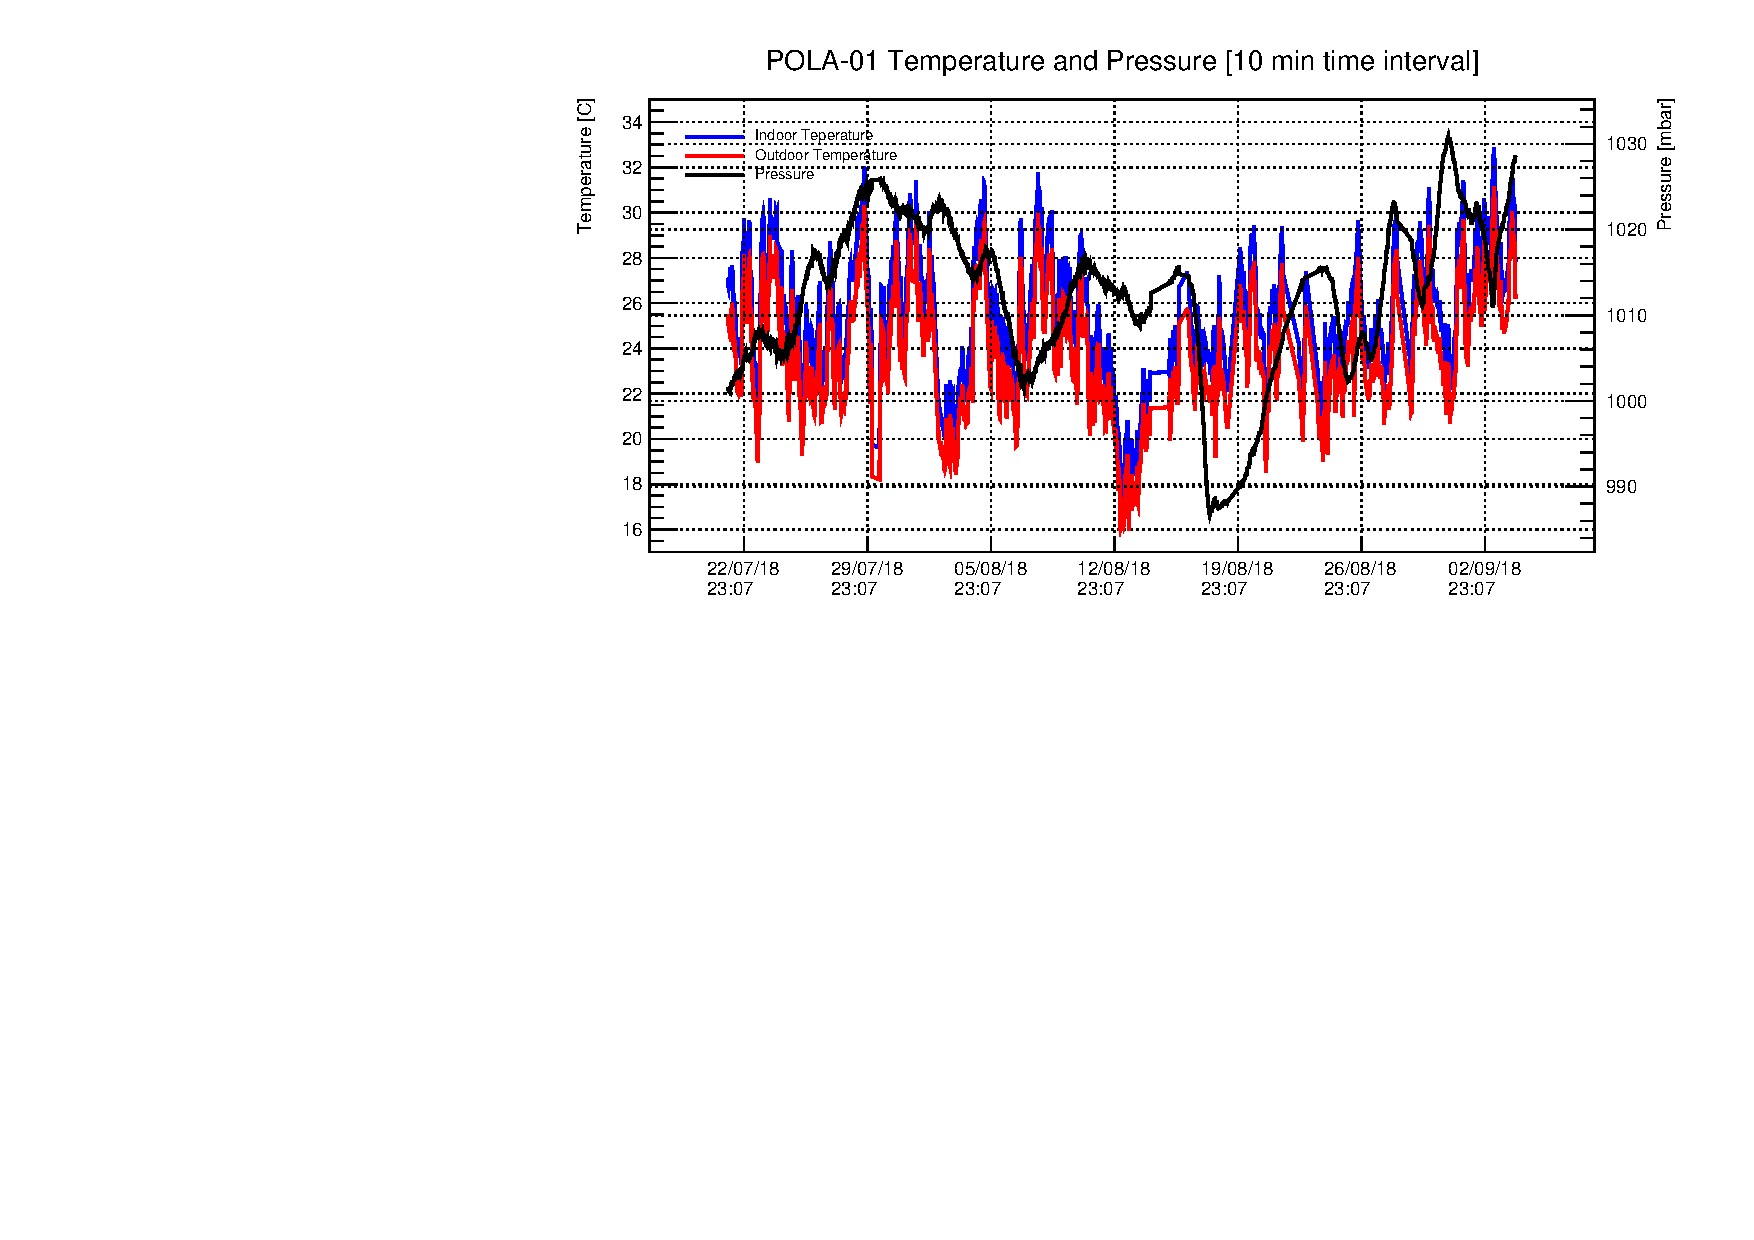
\includegraphics[width=\linewidth]{figures/POLA01_TP.pdf}\label{fig:TP_POLA01}}
    \hspace{0.5cm}
    \subfloat[POLA-02]{ 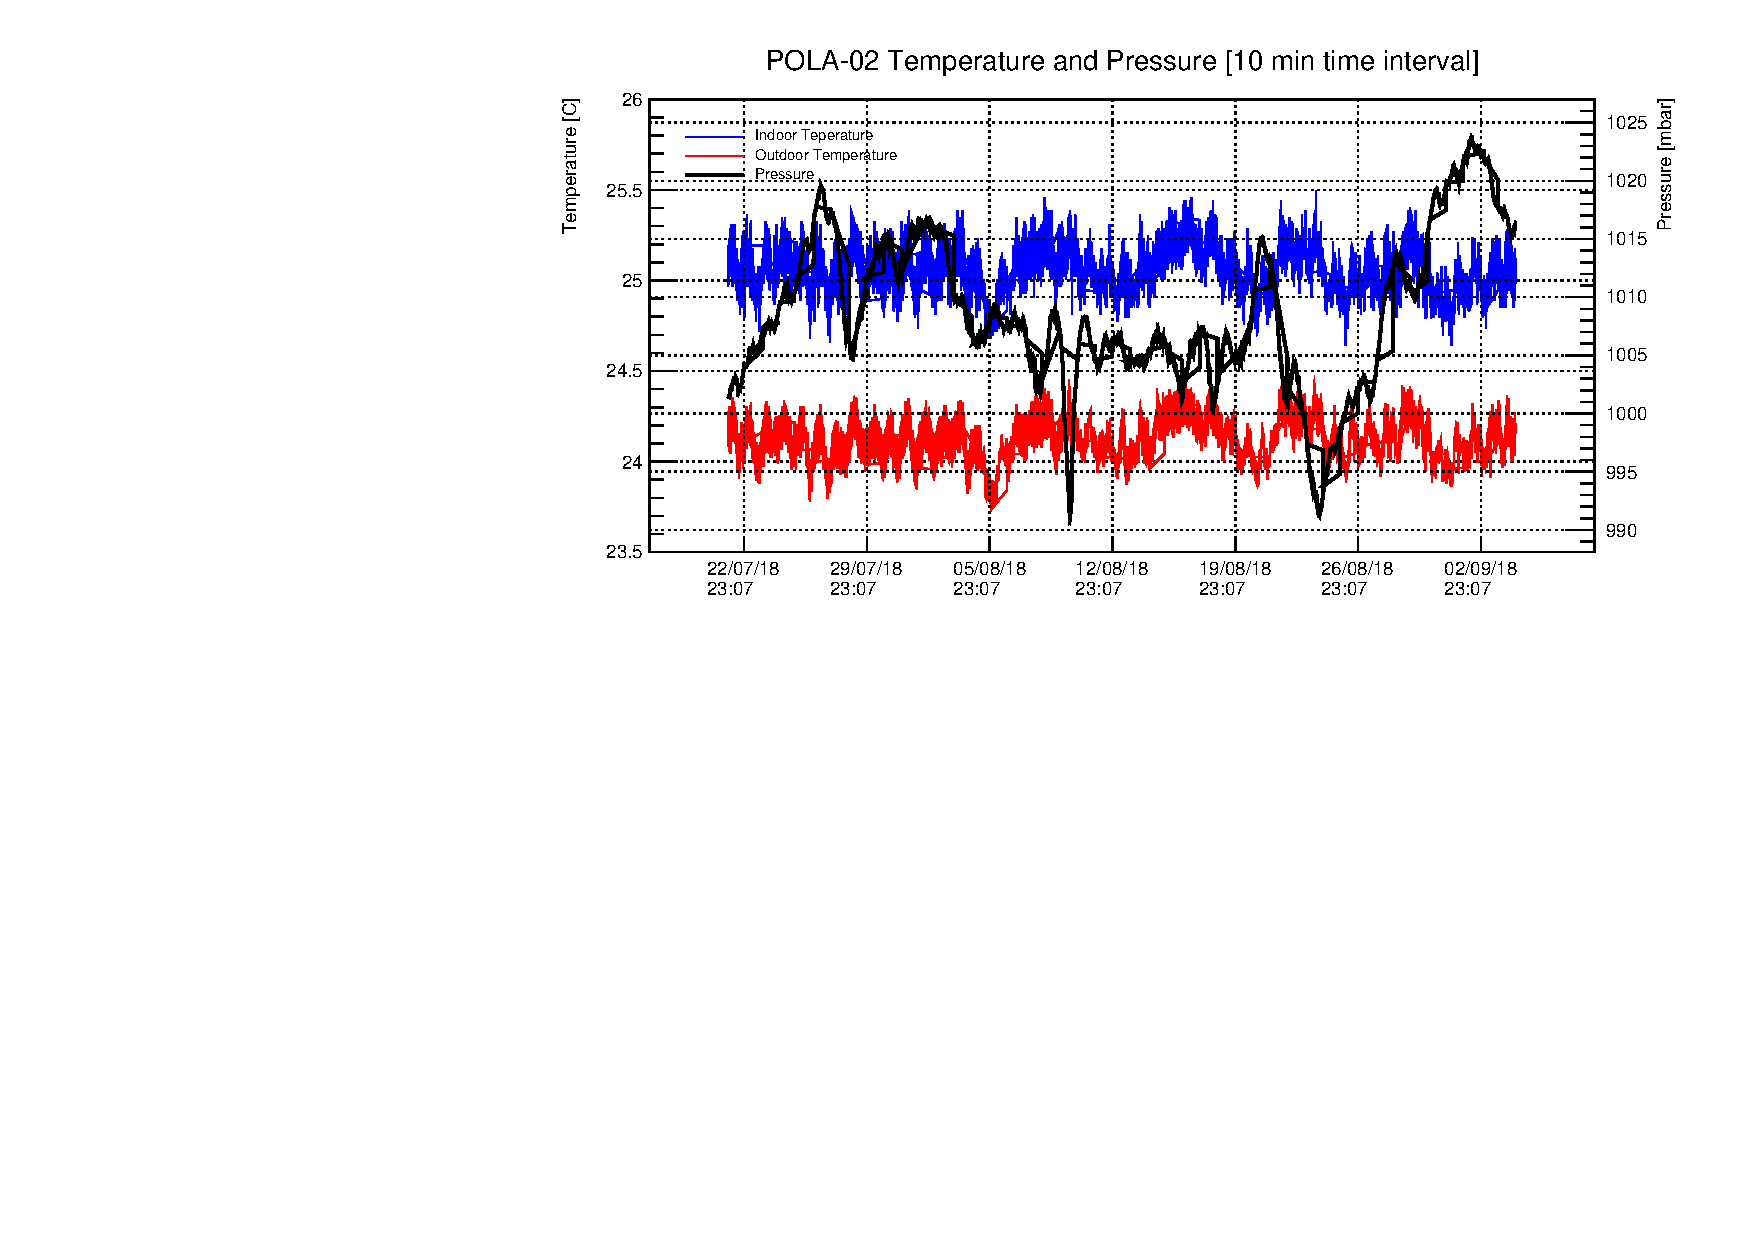
\includegraphics[width=\linewidth]{figures/POLA02_TP.pdf}\label{fig:TP_POLA02}}
    \hspace{0.5cm}
    \subfloat[POLA-03]{ 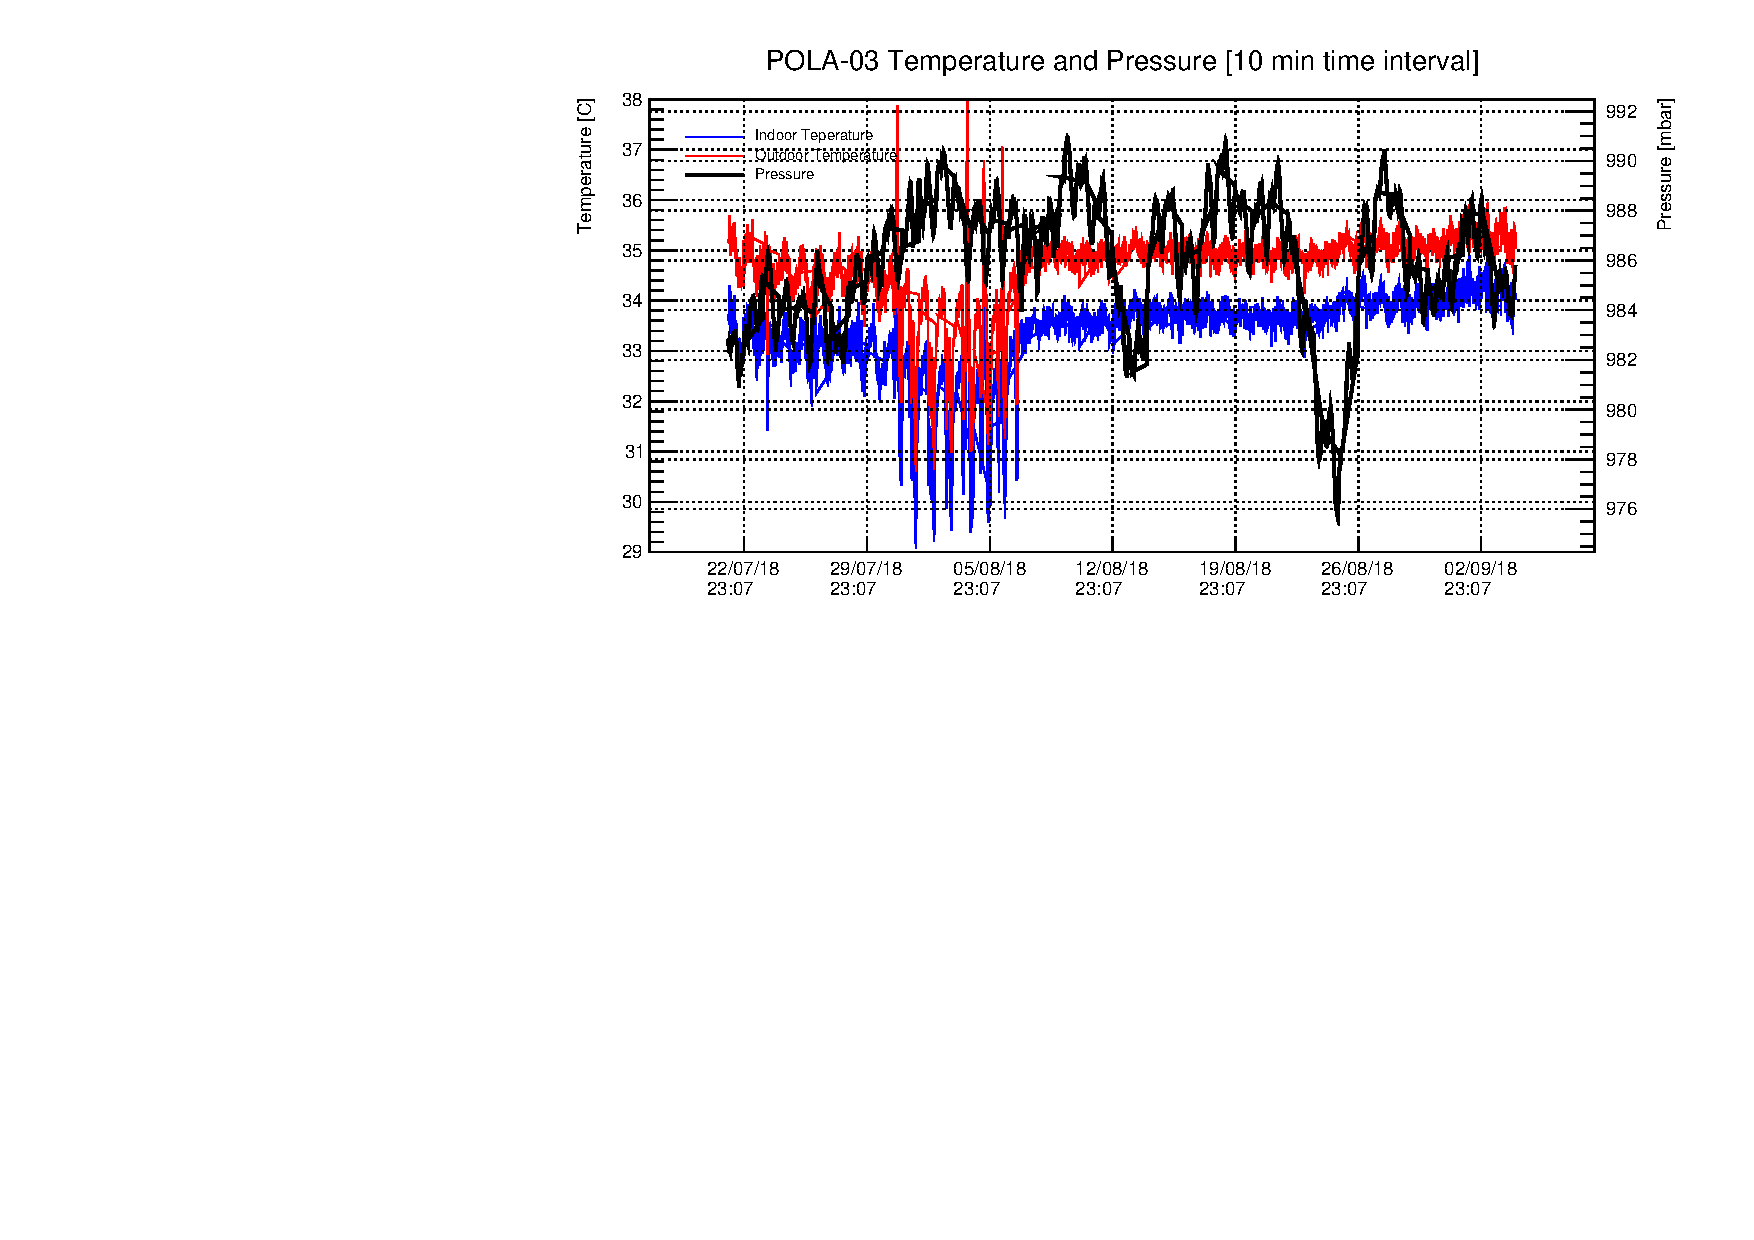
\includegraphics[width=\linewidth]{figures/POLA03_TP.pdf}\label{fig:TP_POLA03}}
    \caption{Temperature and pressure over time for the detectors}
\end{figure}


\subsection{Particle Raw Rate}

The raw rate is defined as raw rate = NumEvents/time. In FIG. \ref{fig:rawrate_time_all} this raw rate is plotted as a function of time for the three detectors. I have removed any outliers that will cause trouble later by applying reasonable cuts on the data if any such points exsists. The raw rate for POLA-01 (black) and POLA-02 (red) overlap and are around the same range of values while the rate for POLA-03 is lower. This is explained in \cite{EEEcosmicrays} as a result of the presence of dense material on the roof above the detector.For both POLA-02 and POLA-03 we can see a large deviation in pressure around 26/08/18, in this time period the raw rates also deviate quite alot. 

\begin{figure}
    \centering
    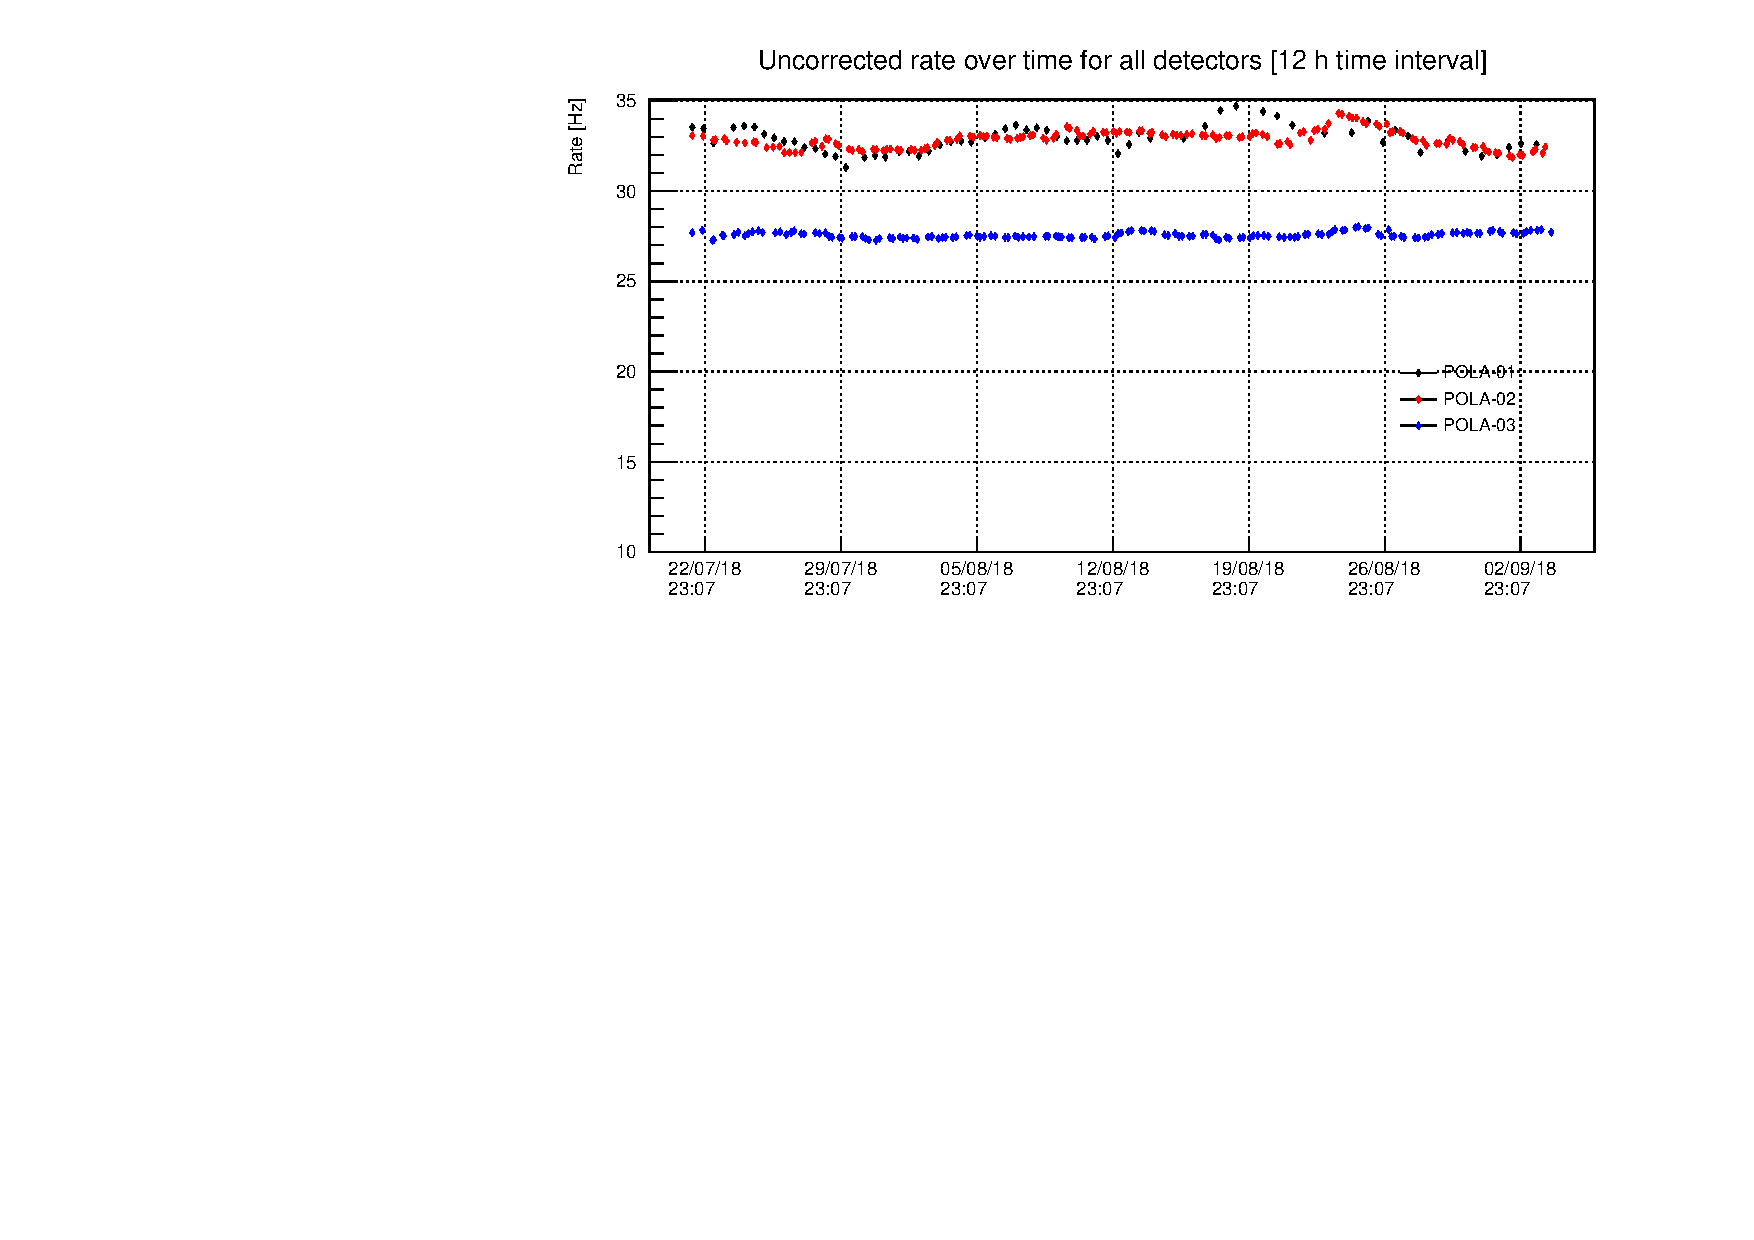
\includegraphics[width=\linewidth]{figures/all_raw3_fixed.pdf}
    \caption{Uncorrected raw rate over time for all three detectors.}
    \label{fig:rawrate_time_all}
\end{figure}

\subsubsection{Longitude and Latitude}

The latitude and longitude of POLA-01 are shown in \ref{fig:coord_POLA01}. This can be compared to the image from the article \cite{EEEcosmicrays} shown in FIG. \ref{fig:from_paper}. FIG. \ref{fig:rate_coord_time_01} shows the raw rate as a function of longitude and latitude.

\begin{figure}
    \centering
    \subfloat[Computed]{
    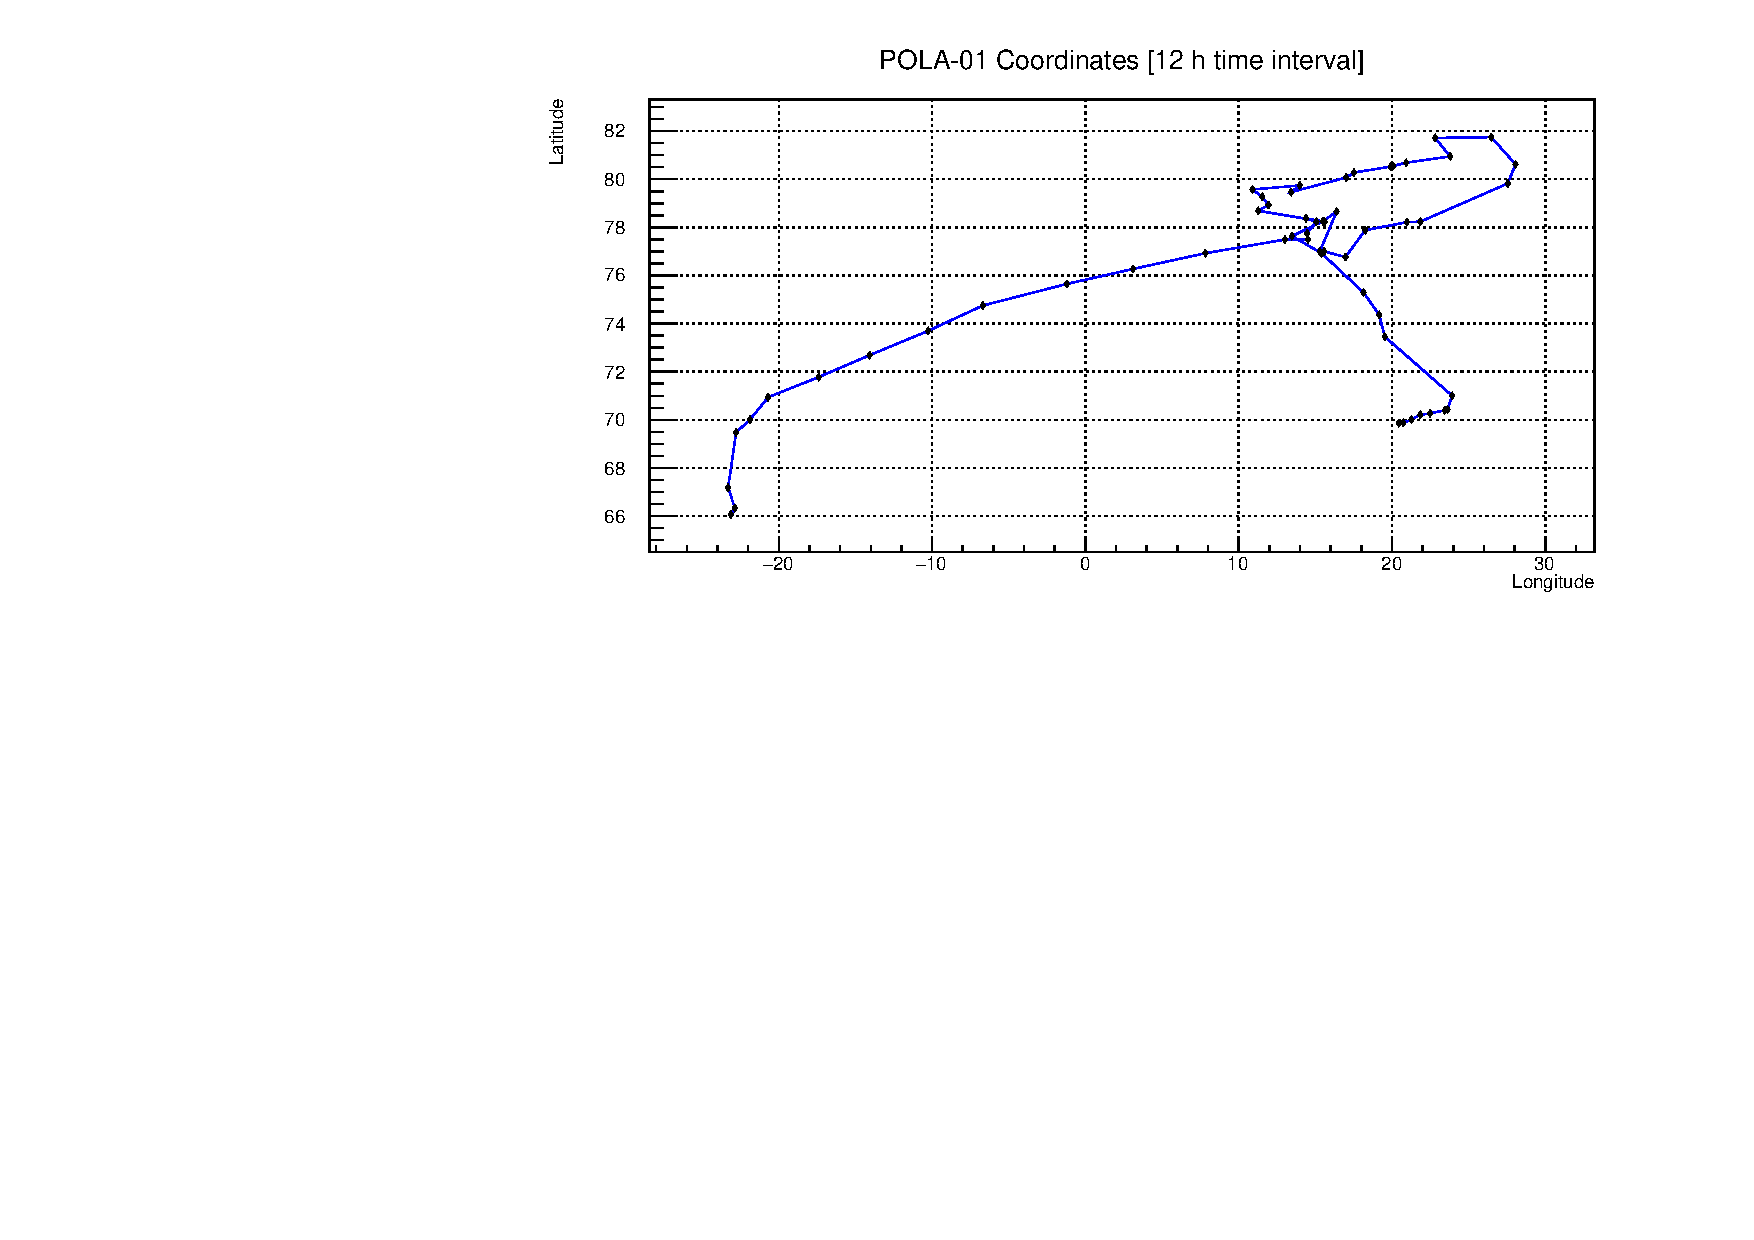
\includegraphics[width=0.5\linewidth]{figures/POLA01_lat_long.pdf}
    \label{fig:coord_POLA01}}
    \subfloat[From article]{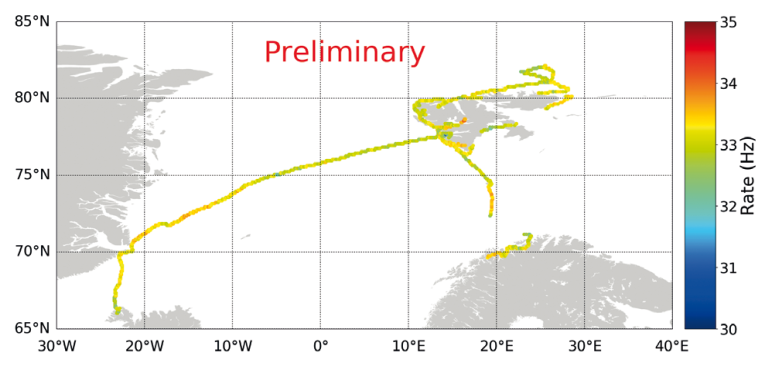
\includegraphics[width = 0.5\linewidth]{figures/cordinates_paper.png}
    \label{fig:from_paper}}
    \caption{a) Computed latitude and Longitude for the POLA-01 detector, both latitude and longitude is given in decimal coordinates. b) The voyage of Nanuq in longitude-latitude plane, displaying, in colour, the different preliminary rates measured by POLA-01, after pressure and vertical angle corrections-image from \cite{EEEcosmicrays}}
    \label{fig:coordinates_POLA01_ab}
\end{figure}

\begin{figure}
    \centering
    \subfloat{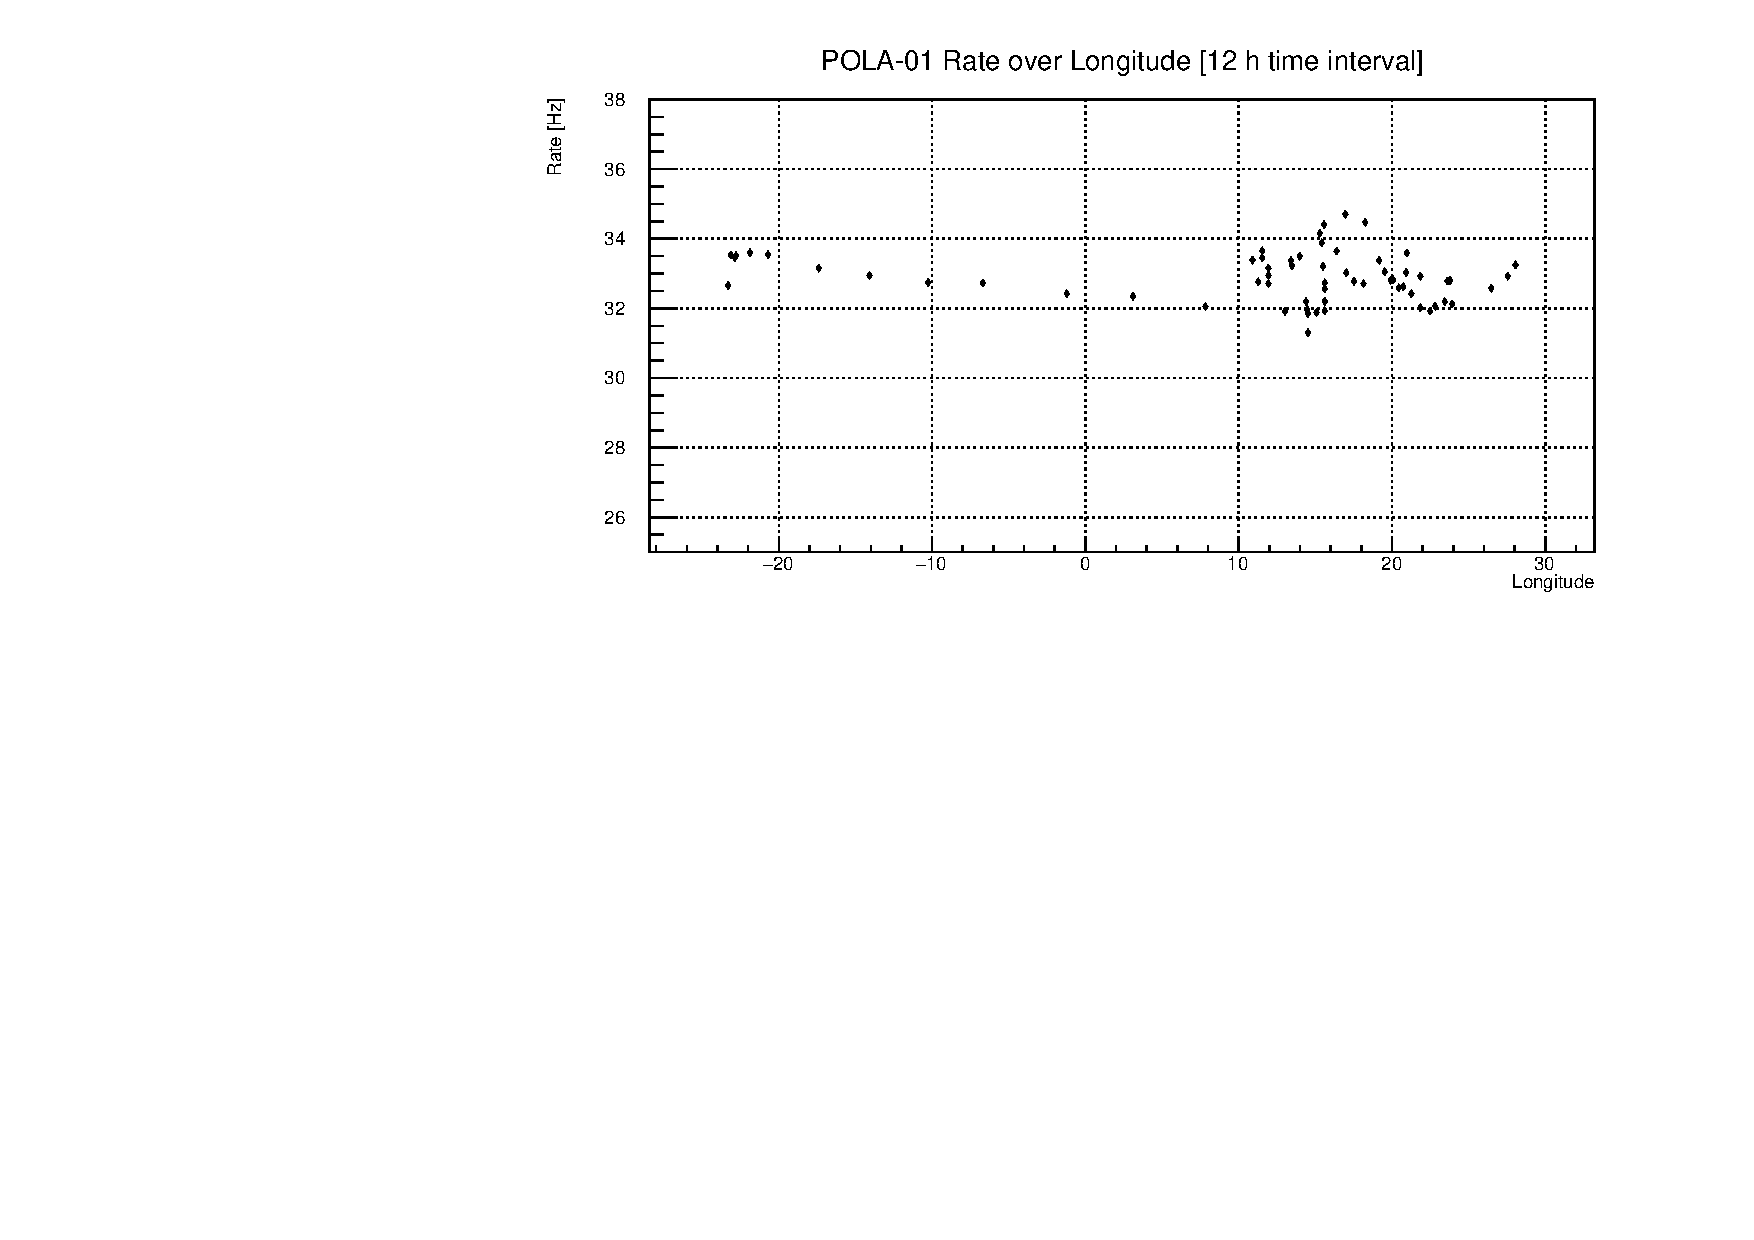
\includegraphics[width=\linewidth]{figures/POLA01_raw_coordinate_Longitude.pdf}\label{fig:rate_long_time_01}}
    \hspace{0.5cm}
    \subfloat{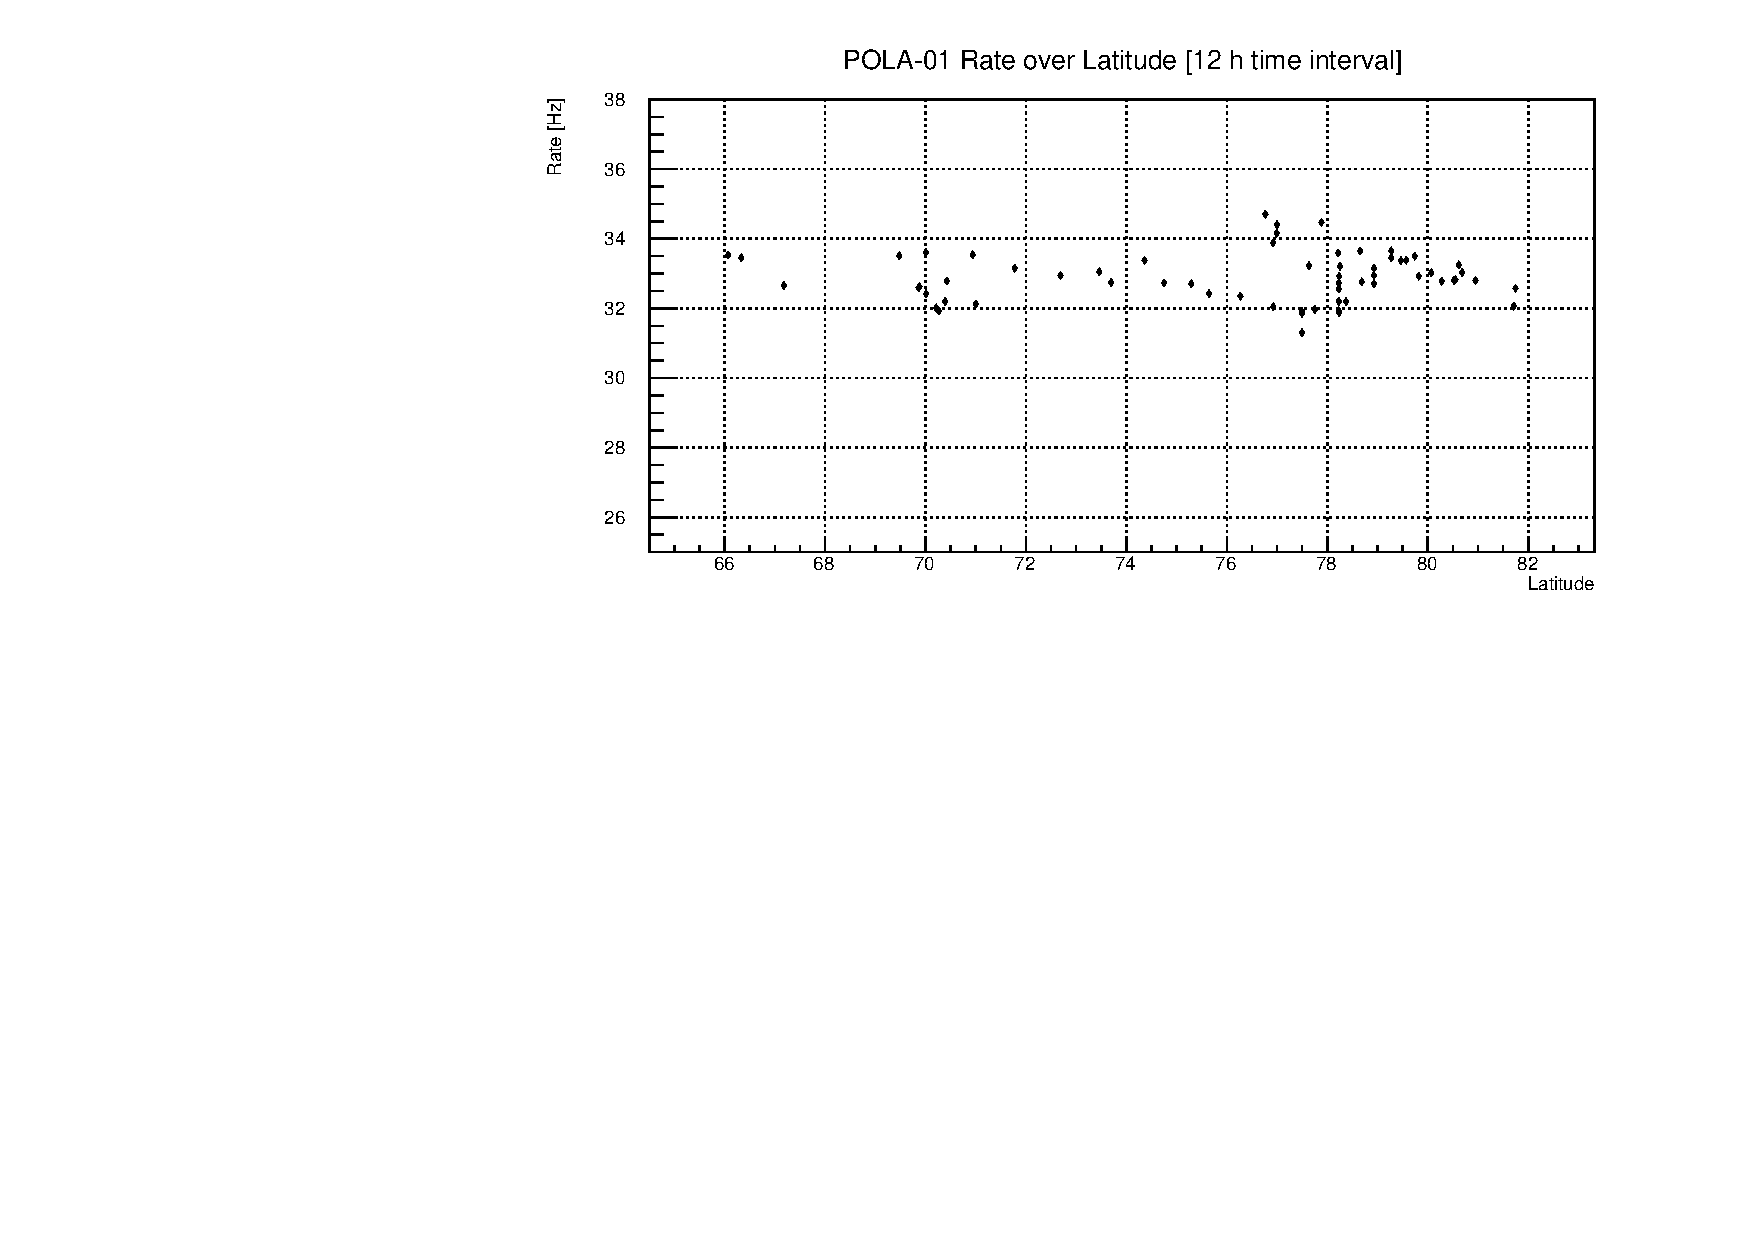
\includegraphics[width=\linewidth]{figures/POLA01_raw_coordinate_Latitude.pdf}\label{fig:rate_lat_time_01}}
    \caption{Change in raw rate and longitude/latitude over time for POLA-01.}\label{fig:rate_coord_time_01}
\end{figure}

\subsubsection{Barometric Correction coefficients}

The change in rate caused by changes in the pressure is experimentally shown to have an exponential dependence which to first order approximation\cite{Kobelev} \cite{doi:10.1029/2012JA018026} can be expressed as, 

\begin{align}
    \frac{\Delta I}{I} \approx \beta \cdot \Delta P
\end{align}

where $\Delta P = P-P_ref$ and $\beta$ is the barometric coefficient. This coefficient is found by following the description from the EEE website \cite{EEEwebsite} by plotting raw rate vs pressure and doing a linear fit to the data. The barometric coefficient is then

\begin{align}
    \beta = \frac{p1}{\text{avgRawRate}} \cdot 100 [\%/\text{mbar}]
    \label{eq:barometric}
\end{align}

Once we find $\beta$ we retrieve the corrected rate using

\begin{align}
    \text{CorrectedRate} = \text{RawRate}(1-\beta\Delta P)
    \label{eq:corrected_raw}
\end{align}

To calculate the temperature coefficient $\alpha$, multiple methods are described by Berkova et. al in \cite{astra-8-41-2012}. In this analysis no temperature correction is yet applied, so $\alpha = 0$. 

\subsubsection{Pressure and Temperature}

In figures \ref{fig:raw_temp_press_all} the raw rate is plotted as a function on temperature and as a function of pressure. The barometric coefficient is found using EQ. \ref{eq:barometric}, and listed in \ref{tab:barometric} along with the reference pressure for each detector. Within the uncertainty the barometric coefficients for POLA-01 and POLA-02 are the same, while for POLA-03, which was located in Italy, is significantly lower.

\begin{table}
    \centering
    \caption{Barometric coefficients and reference pressure for the detectors.}
    \begin{tabular}{c | c | c | c }
         & POLA-01 & POLA-02 & POLA-03  \\
        \hline
        $p_{\text{ref}}$[mbar] & 1011.85 & 1008.53 & 985.87 \\
        $\beta$ [$\%$/mbar]$\quad$ & $-0.25\pm0.02$ & $-0.207\pm0.008$ & $-0.15\pm 0.01$\\
        \hline
    \end{tabular}
    \label{tab:barometric}
\end{table}

\subsubsection{Corrected Raw Rate}

Figures \ref{fig:corrected_rate_1}-\ref{fig:corrected_rate_3} show the rates before and after using the pressure correction in EQ. \ref{eq:corrected_raw}. In figure \ref{fig:corr_all} the corrected raw rate for all detectors are plotted together. There are still some small sudden deviations in the rates, so it may be necessary to apply a temperature correction for all three detectors, and in the case of POLA-01 a correction due to the detector orientation which may change when sailing. 
\begin{figure}
    \centering
    \subfloat{
    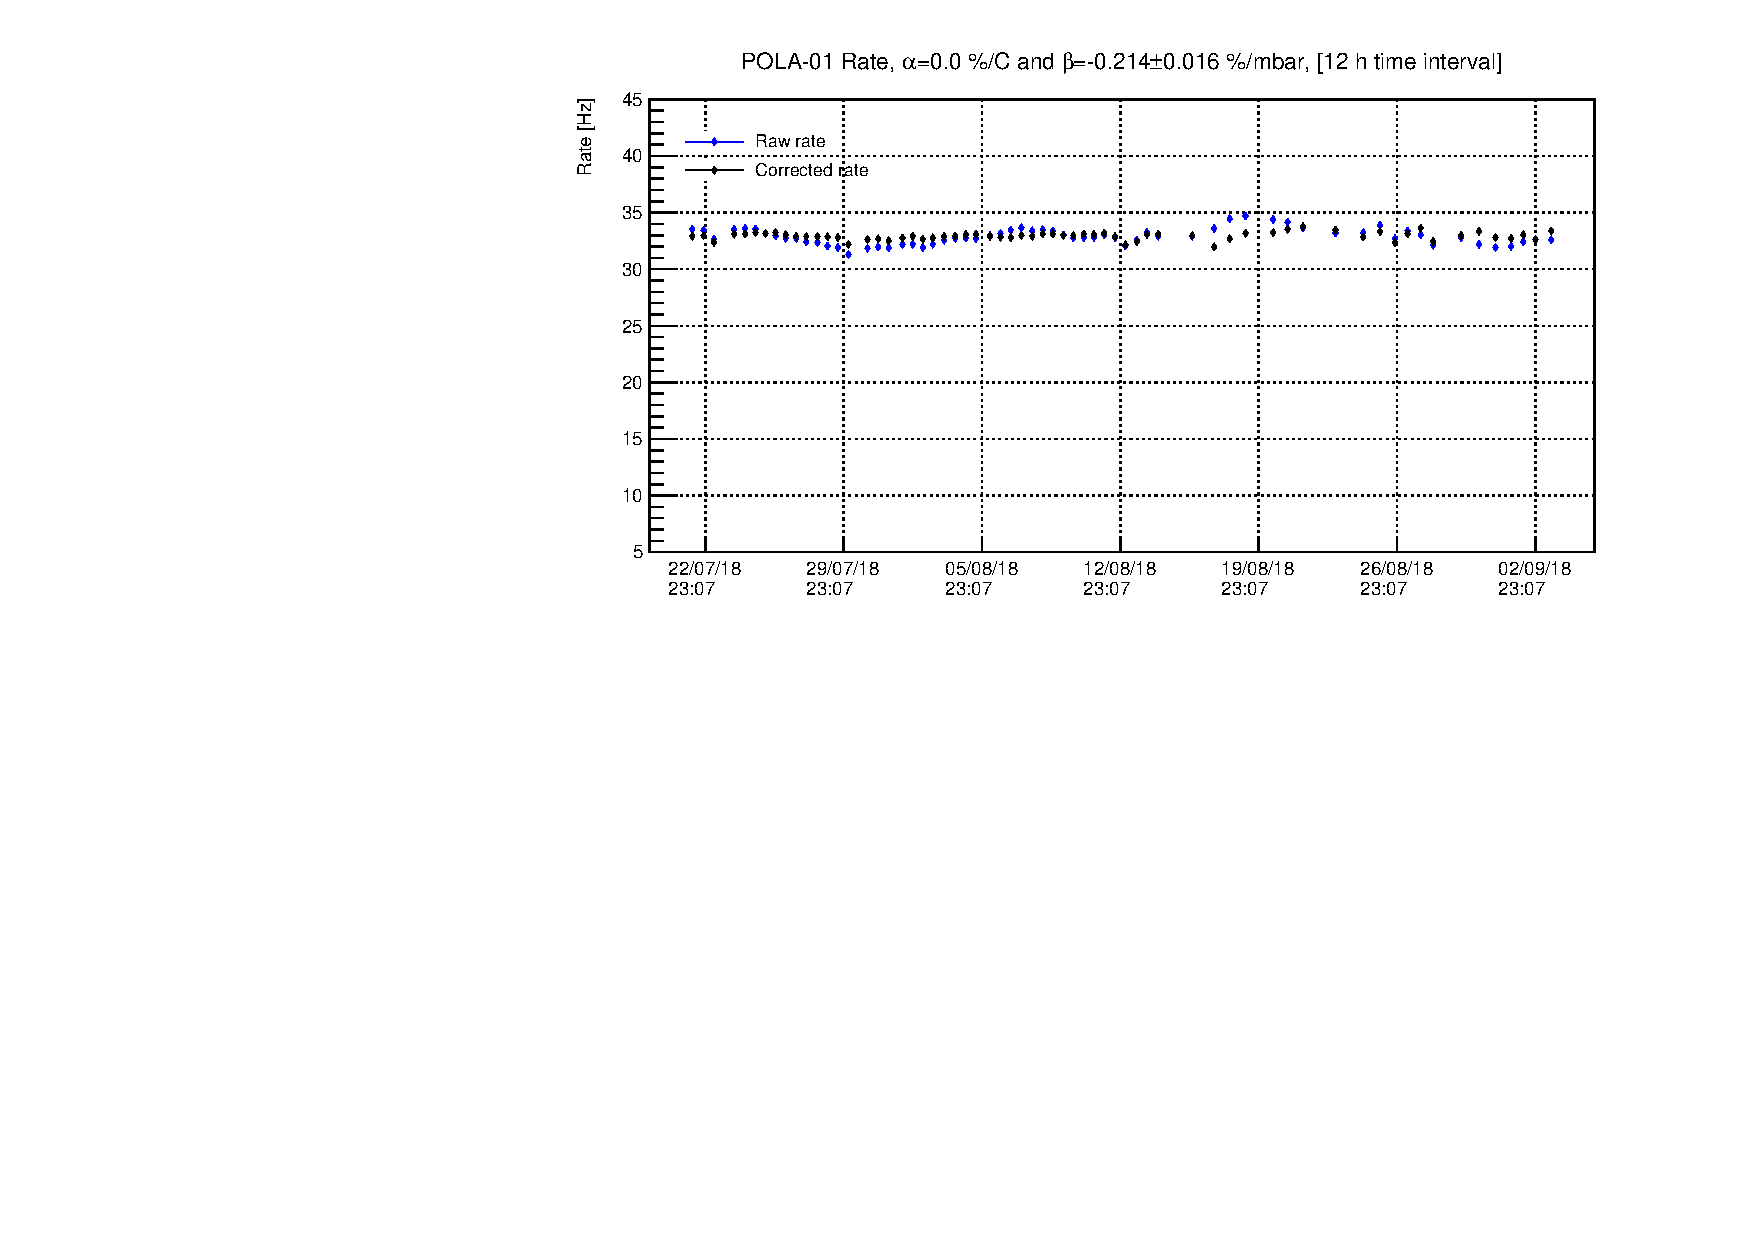
\includegraphics[width=0.9\linewidth]{figures/fixed_POLA01_corrected_rate.pdf}\label{fig:corrected_rate_1}}
    \hspace{0.5cm}
    \subfloat{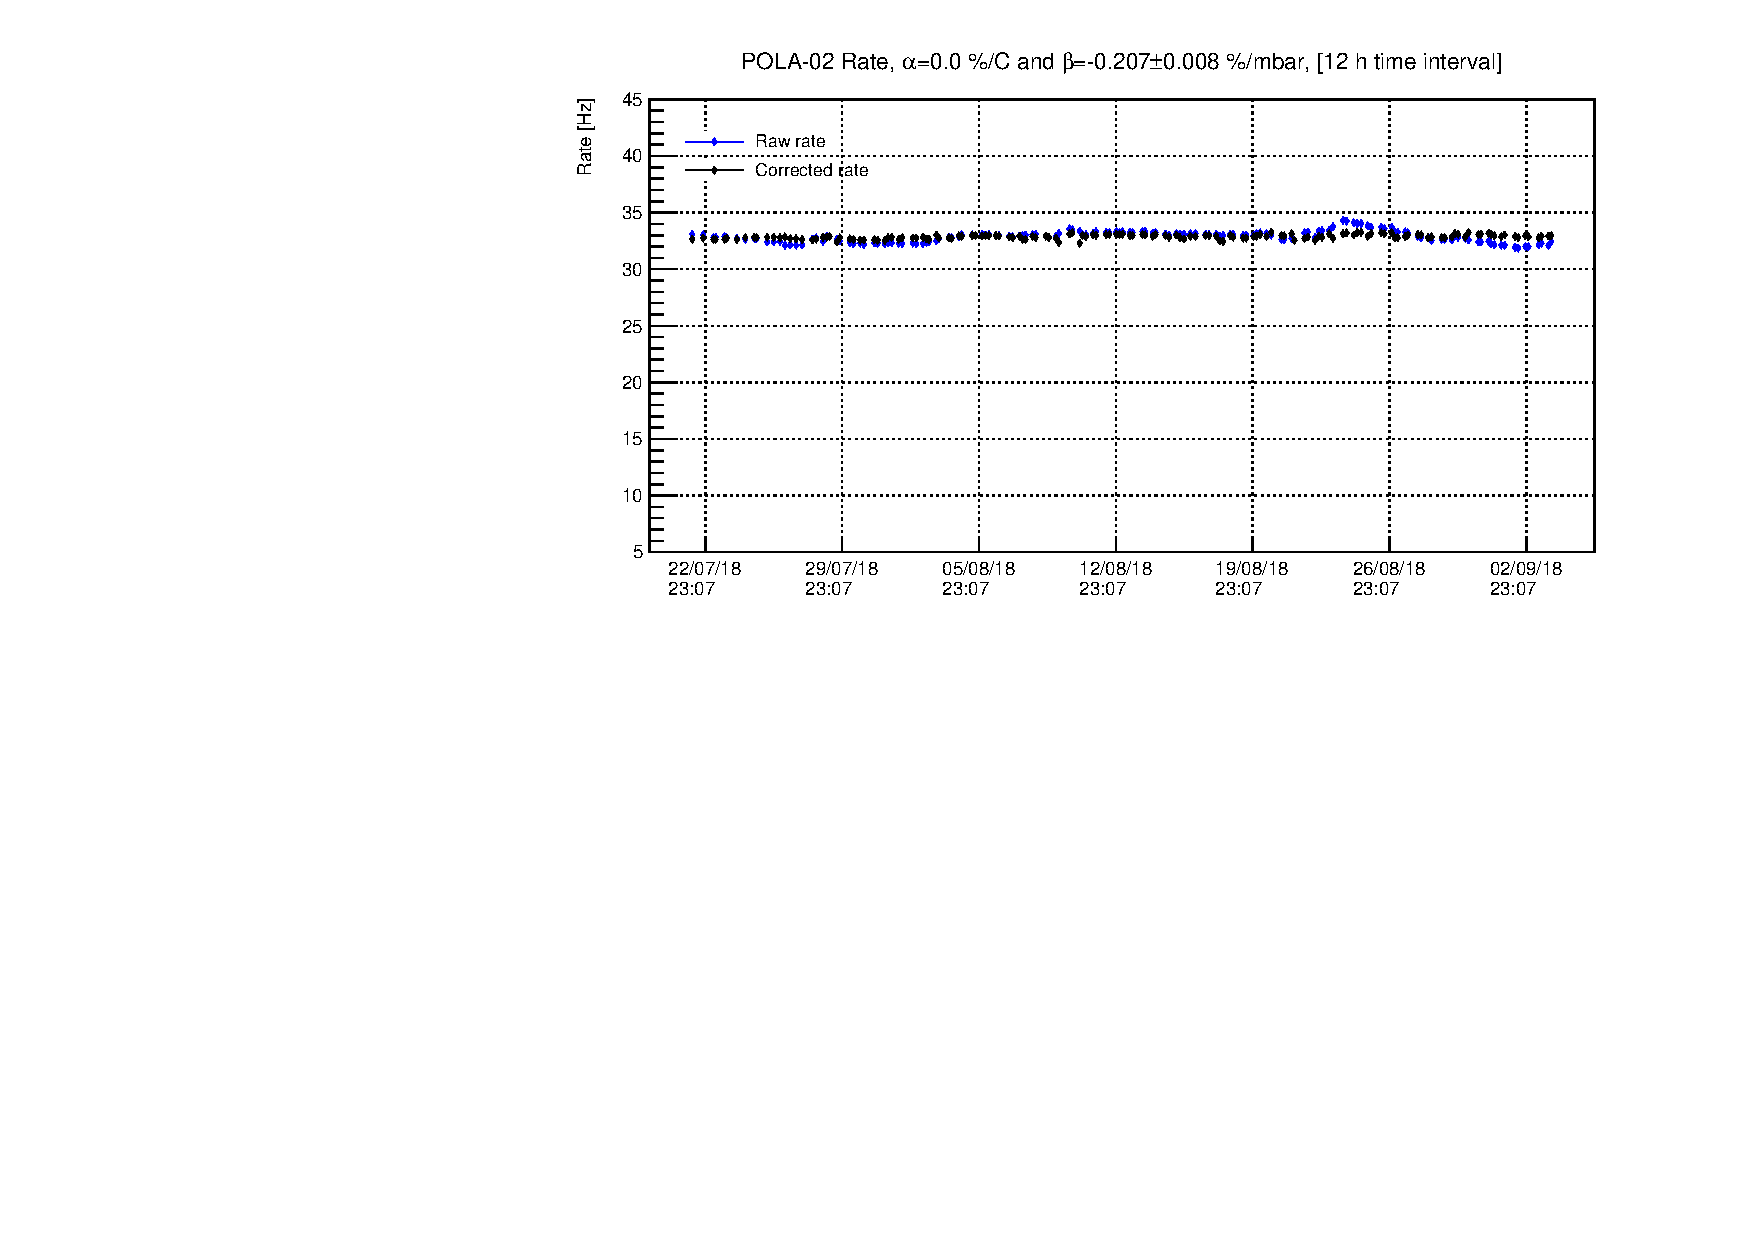
\includegraphics[width=0.9\linewidth]{figures/fixed_POLA02_corrected_rate.pdf}\label{fig:corrected_rate_2}}
    \hspace{0.5cm}
    \subfloat{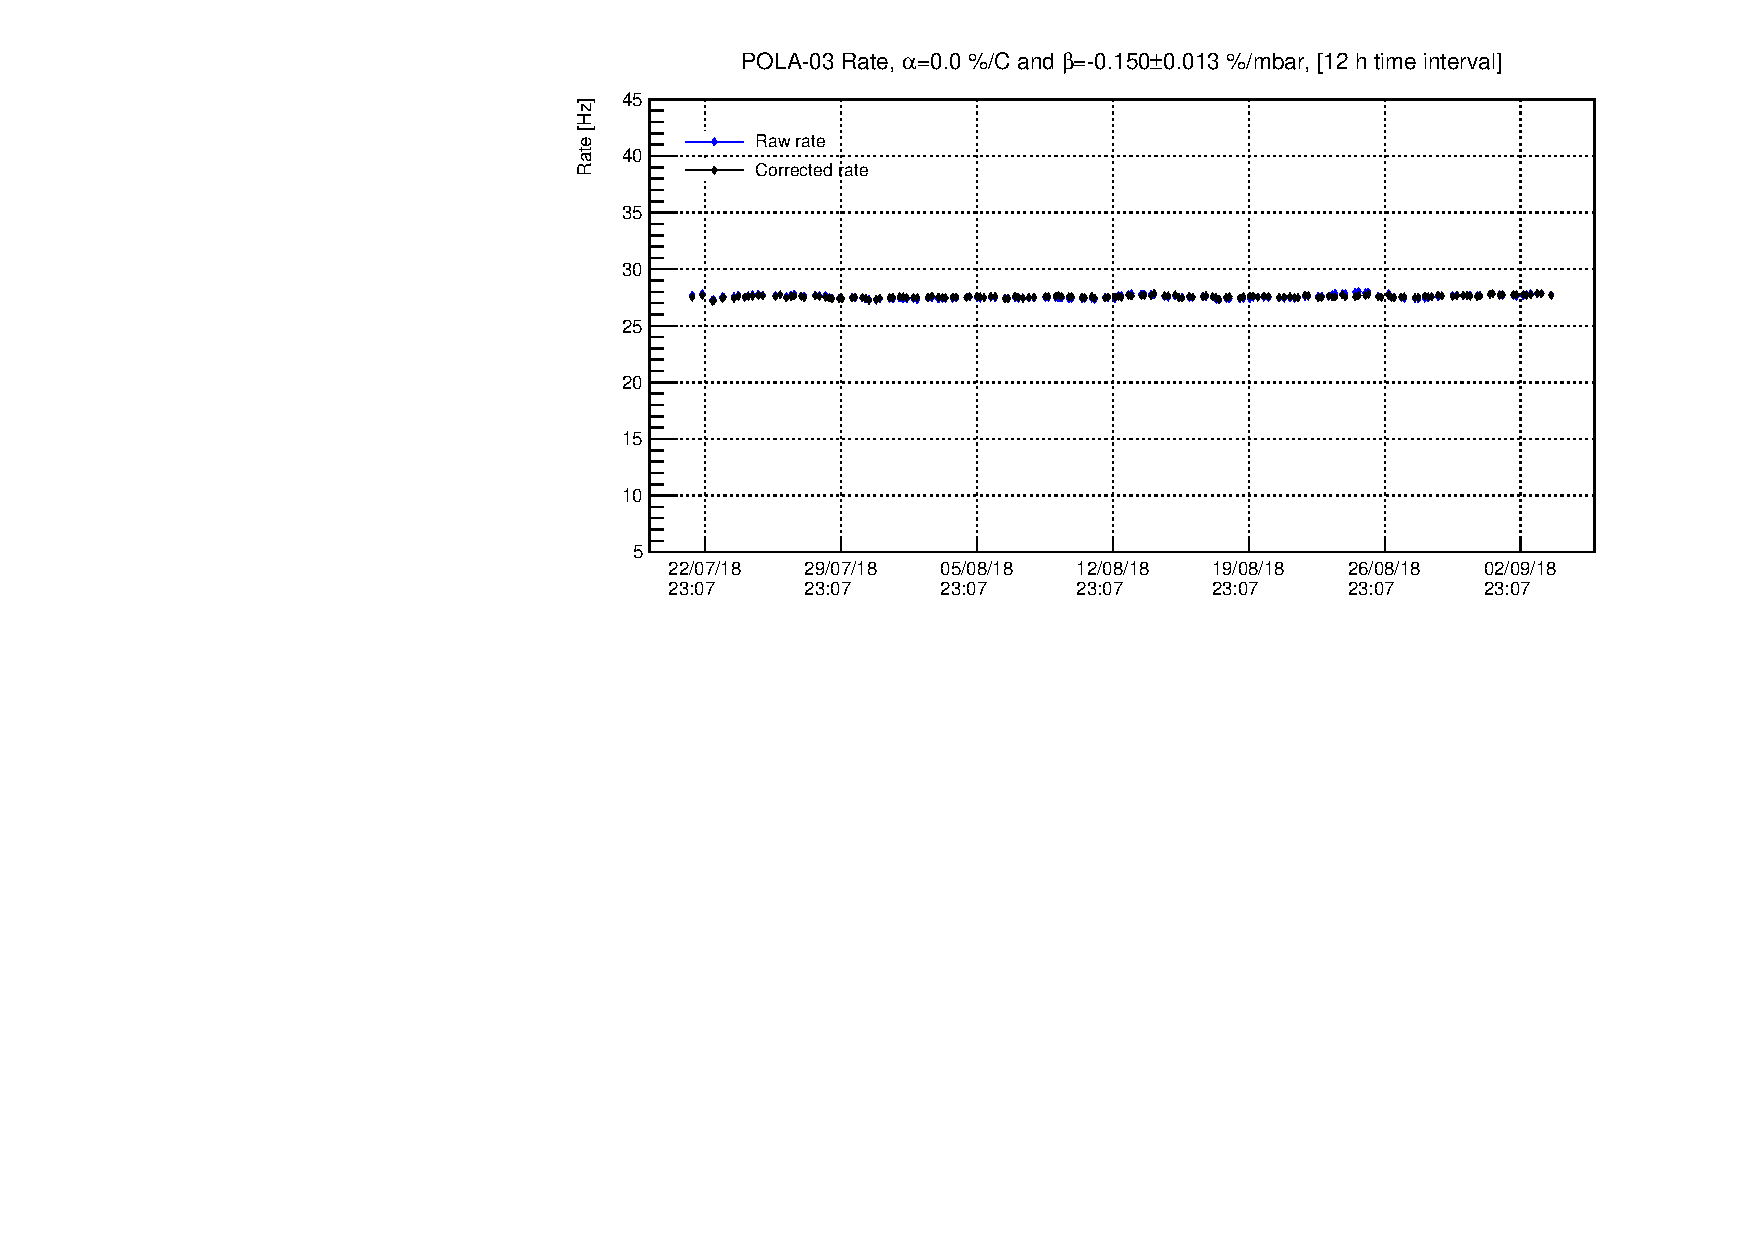
\includegraphics[width=0.9\linewidth]{figures/fixed_POLA03_corrected_rate.pdf}\label{fig:corrected_rate_3}}
    \caption{Uncorrected and corrected rates for the tree detectors.}
\end{figure}

\begin{figure}
    \centering
    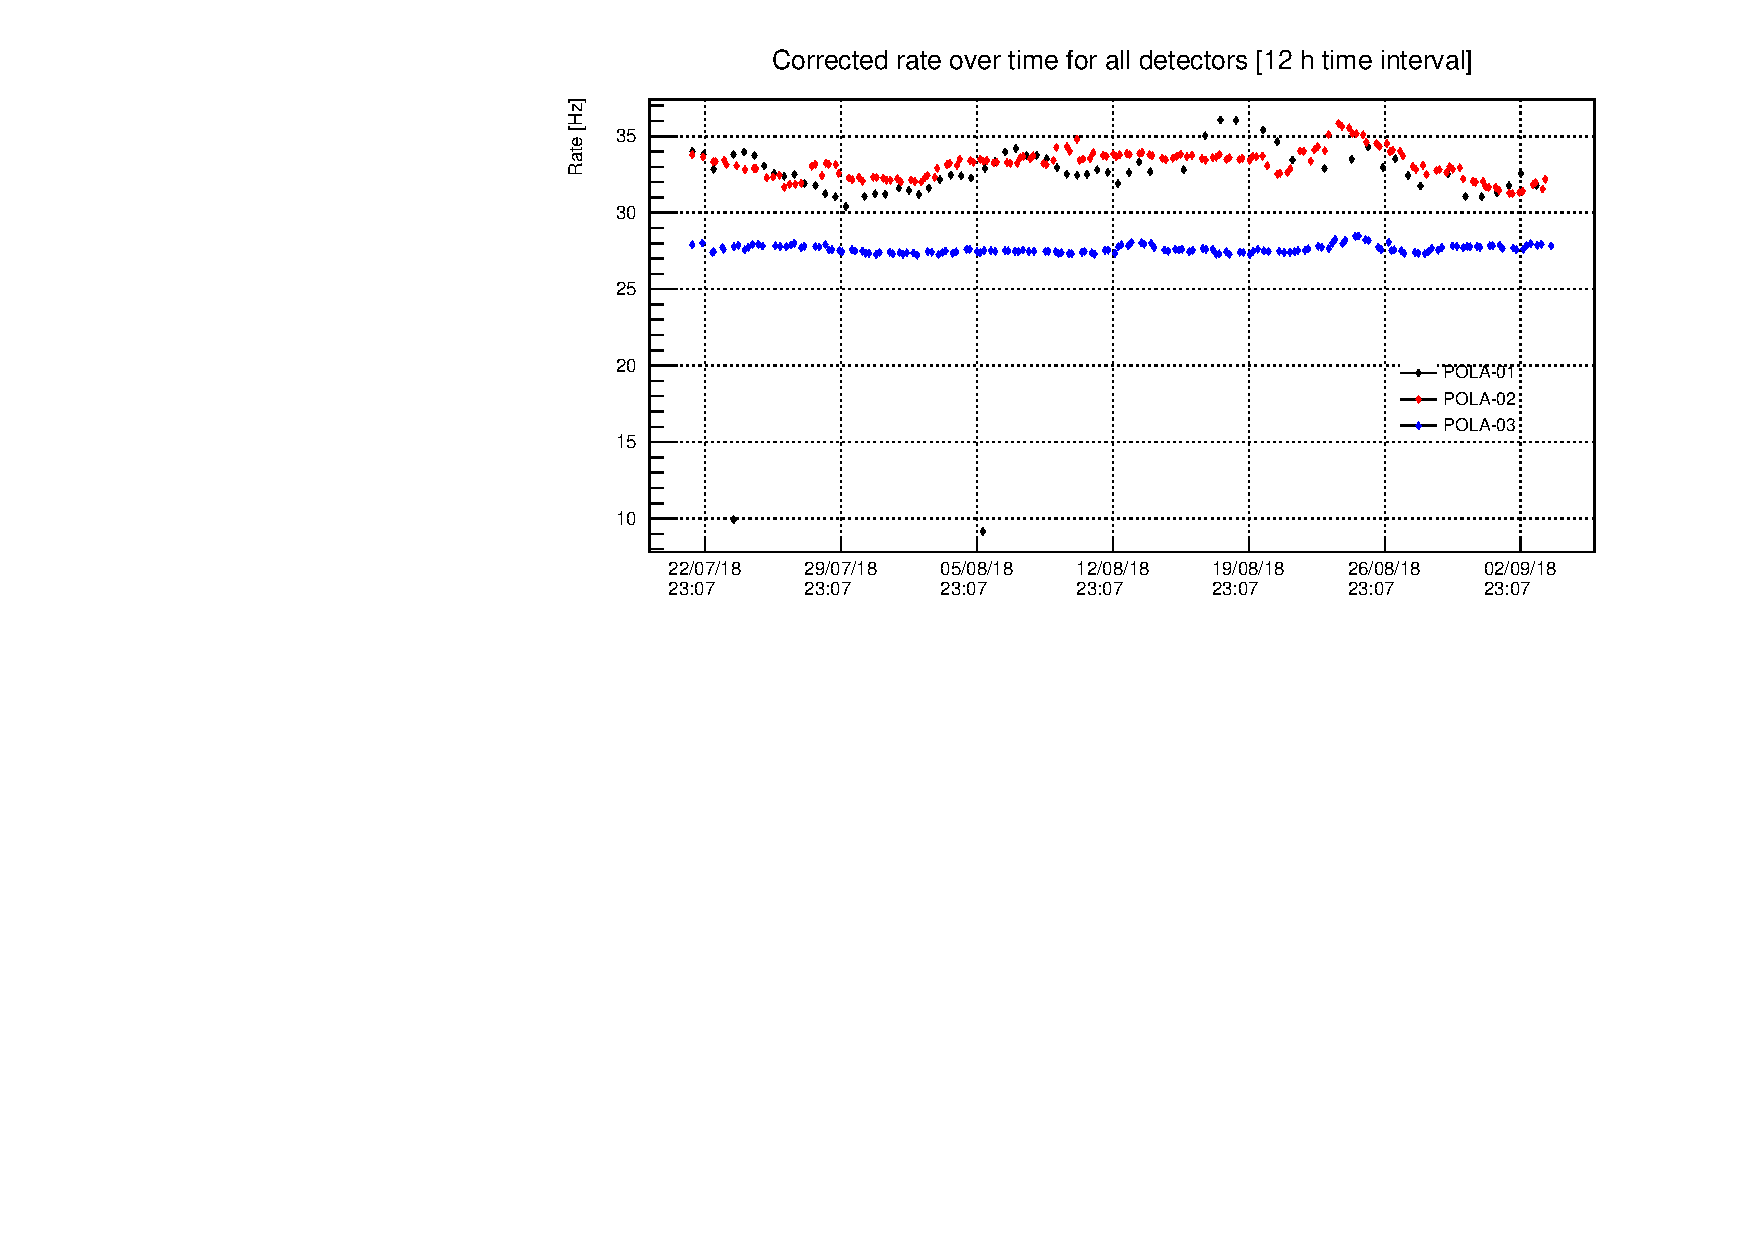
\includegraphics[width =0.9\linewidth]{figures/all_corr3.pdf}
    \caption{Corrected rate for all three detectors.}
    \label{fig:corr_all}
\end{figure}

\onecolumngrid
\newpage
\begin{figure}
    \centering
    \subfloat[POLA-01]{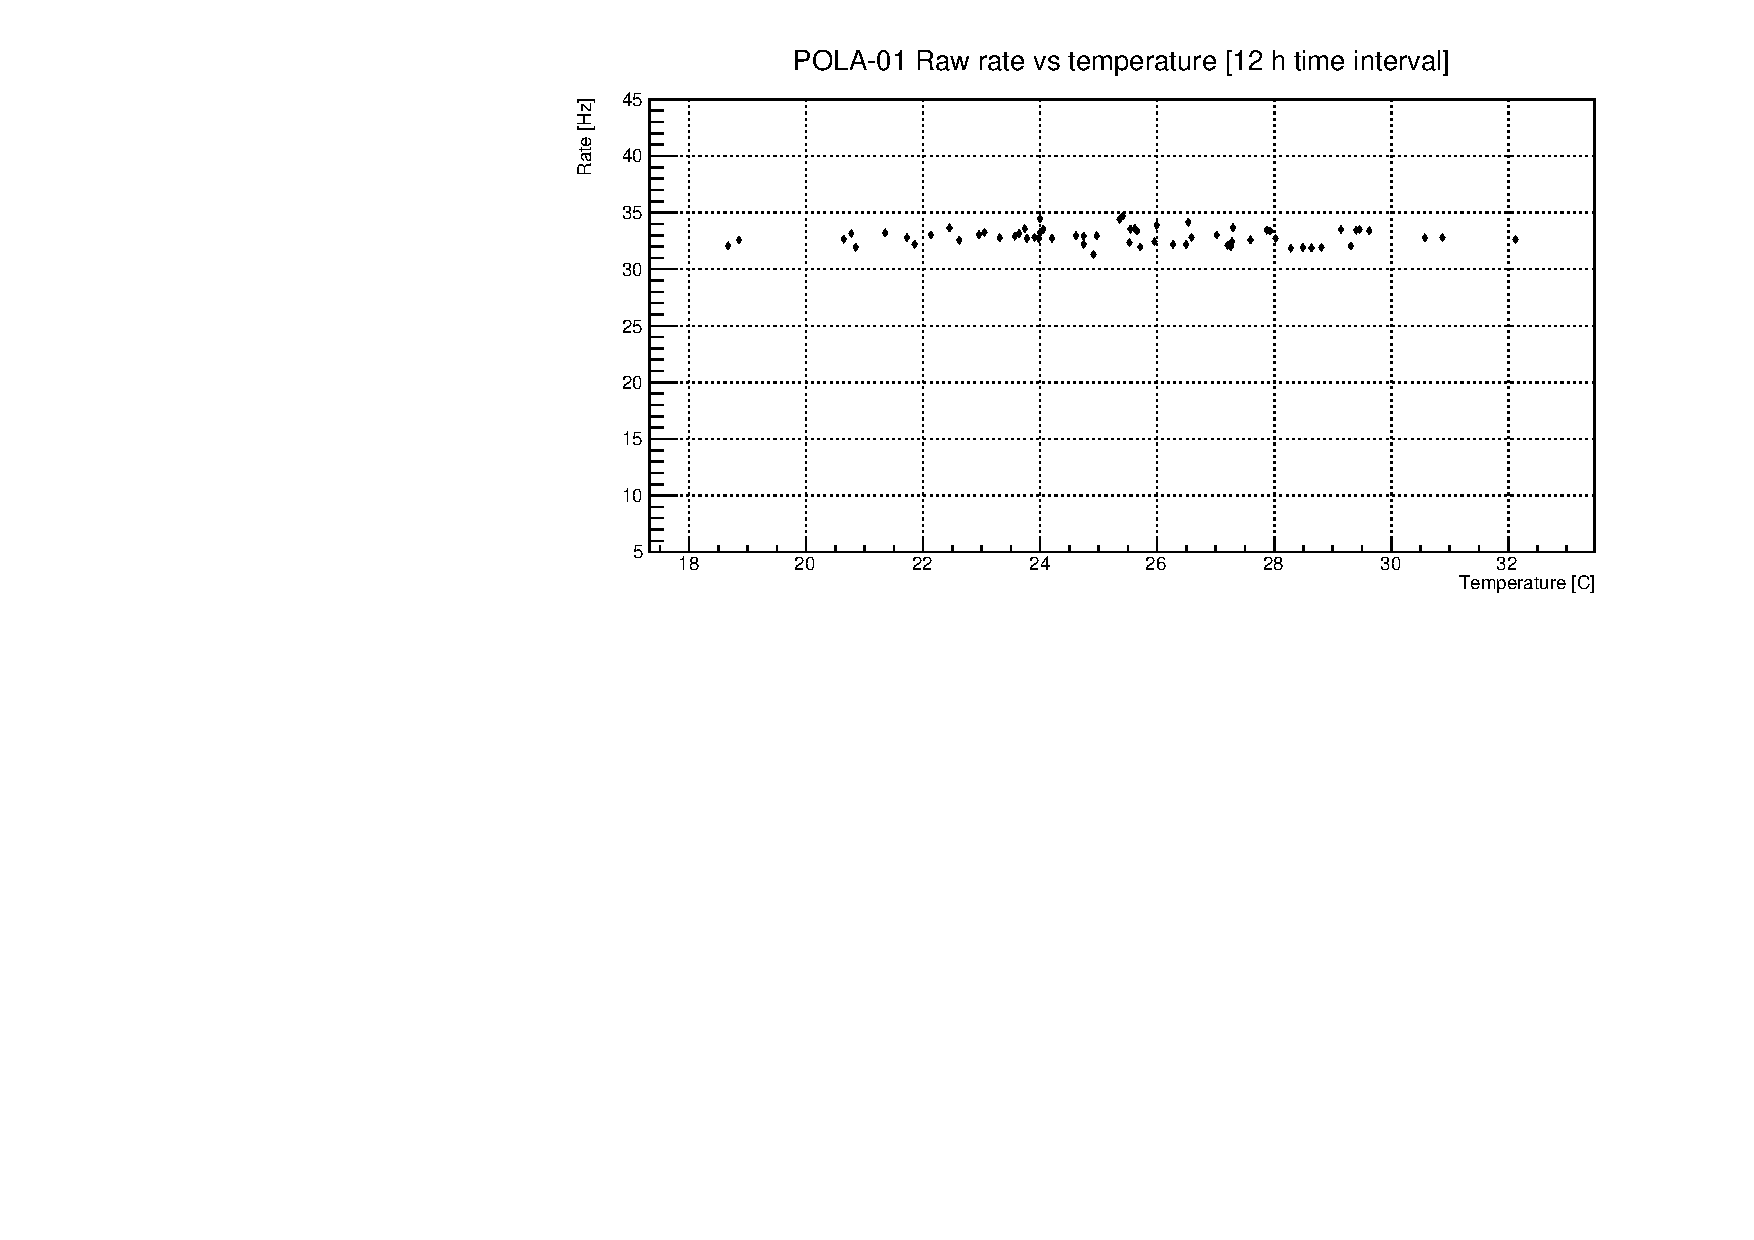
\includegraphics[width=0.5\textwidth]{figures/fixed_POLA01_rate_temp_fit.pdf}}
    \subfloat[POLA-01]{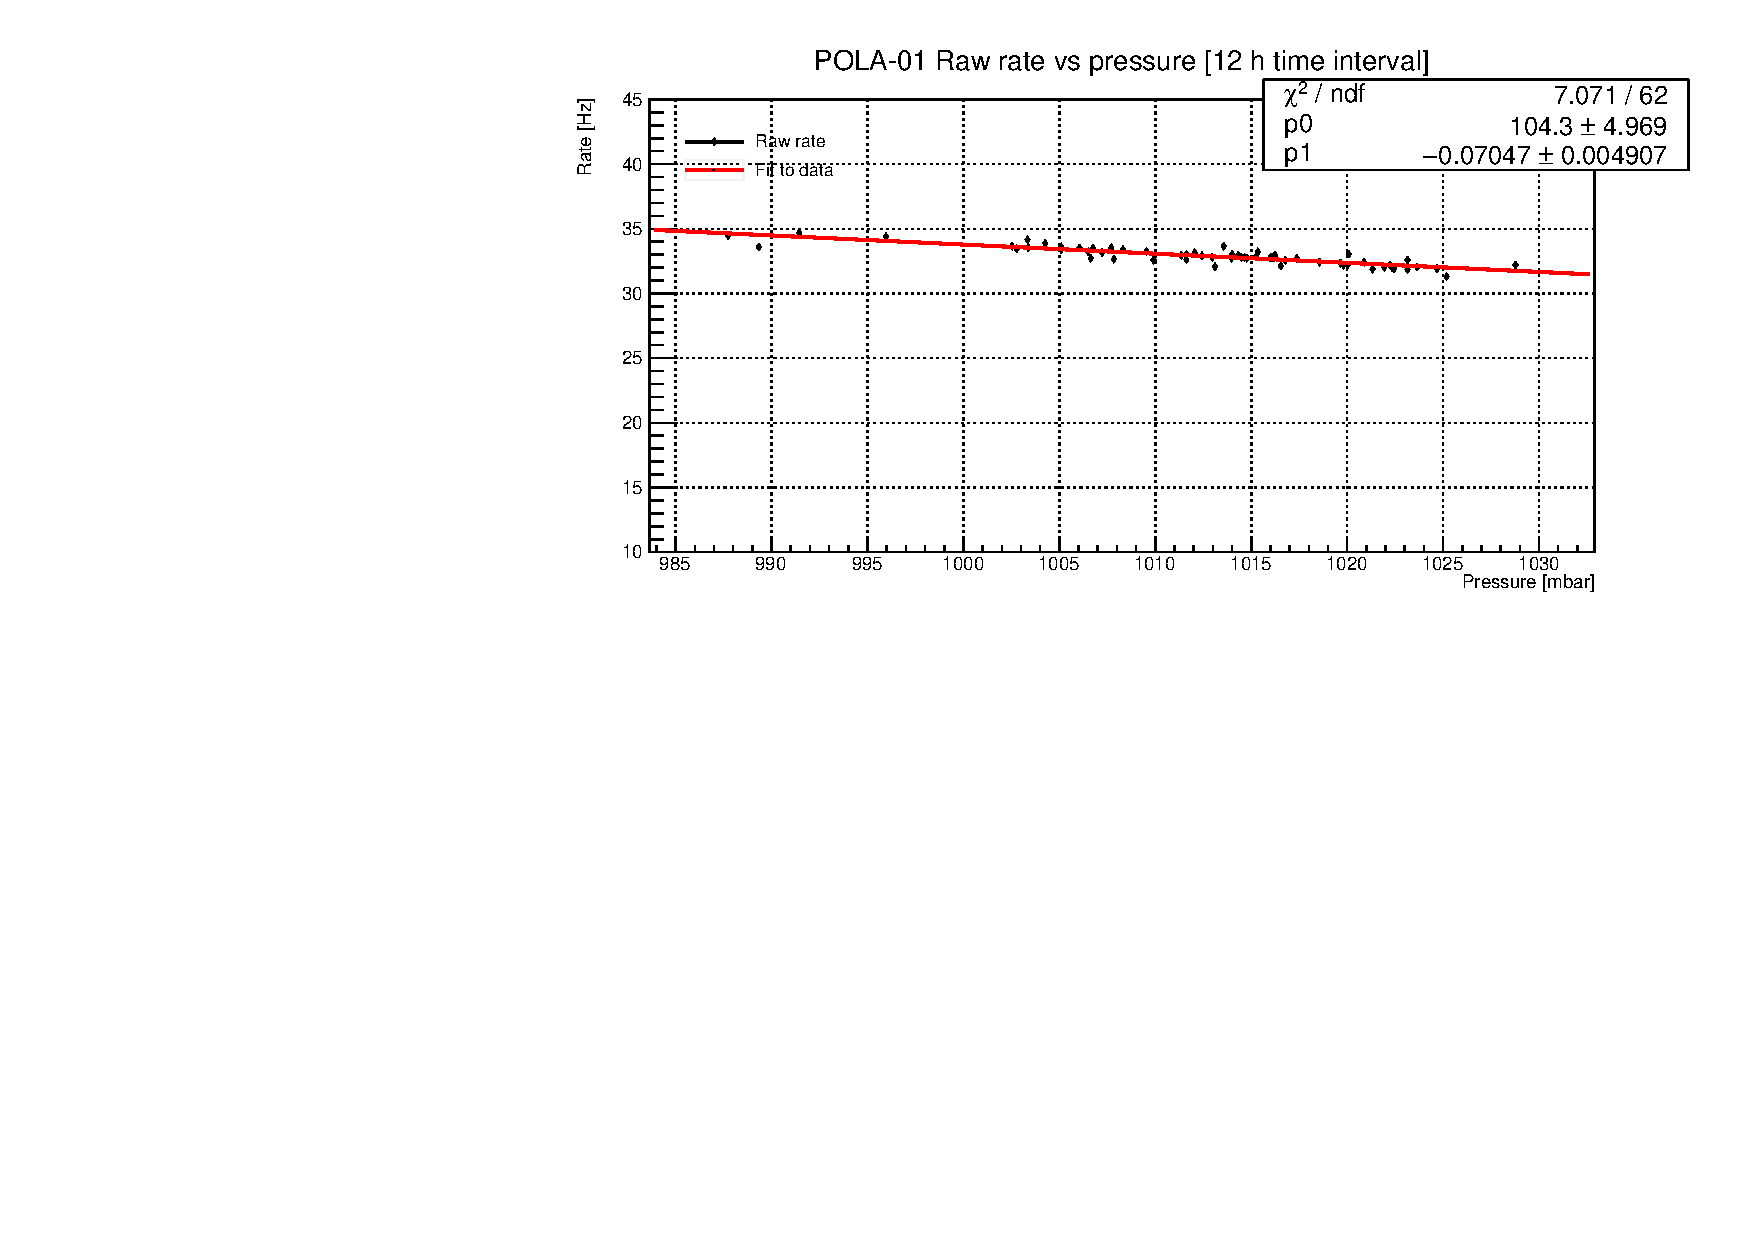
\includegraphics[width=0.5\textwidth]{figures/fixed_POLA01_rate_pressure_fit.pdf}}
    \hspace{0.5cm}
    \subfloat[POLA-02]{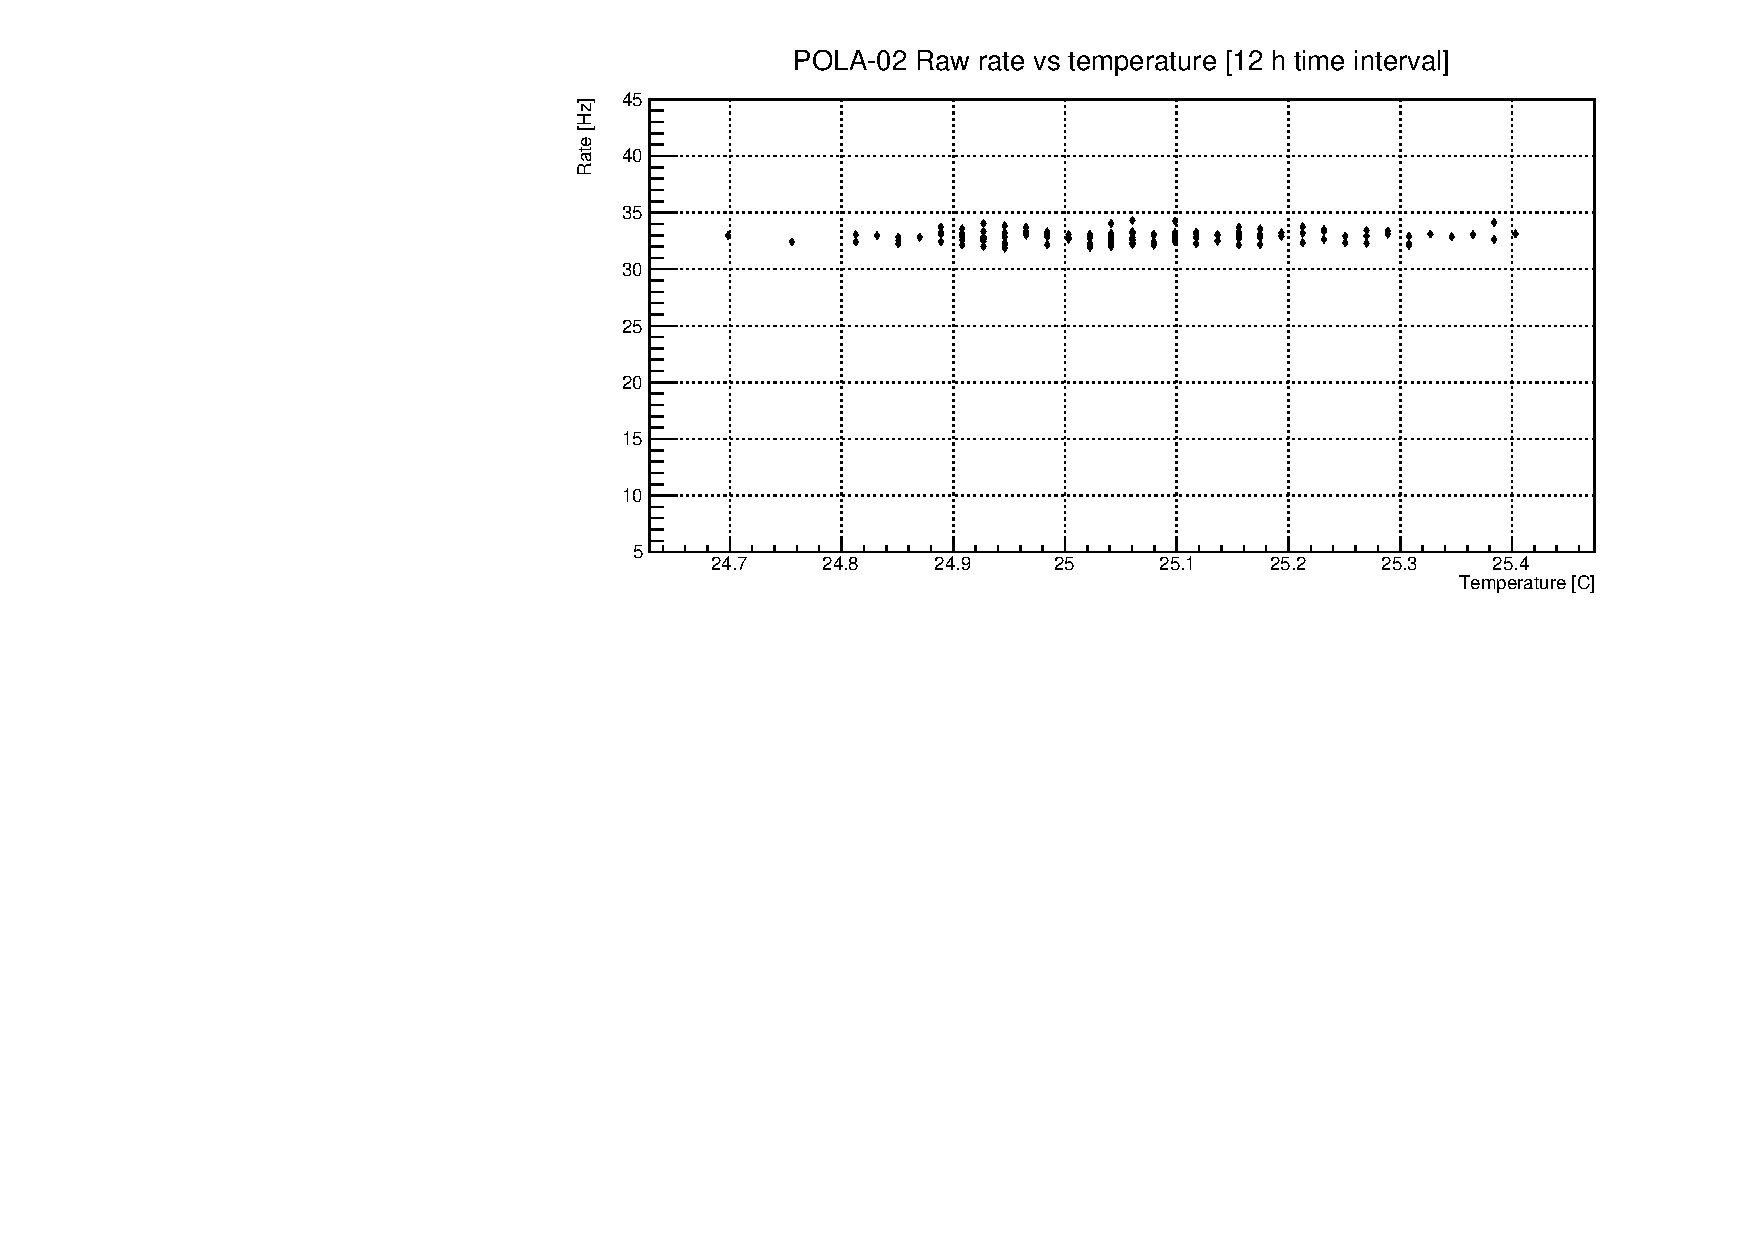
\includegraphics[width=0.5\textwidth]{figures/fixed_POLA02_rate_temp_fit.pdf}}
    \subfloat[POLA-02]{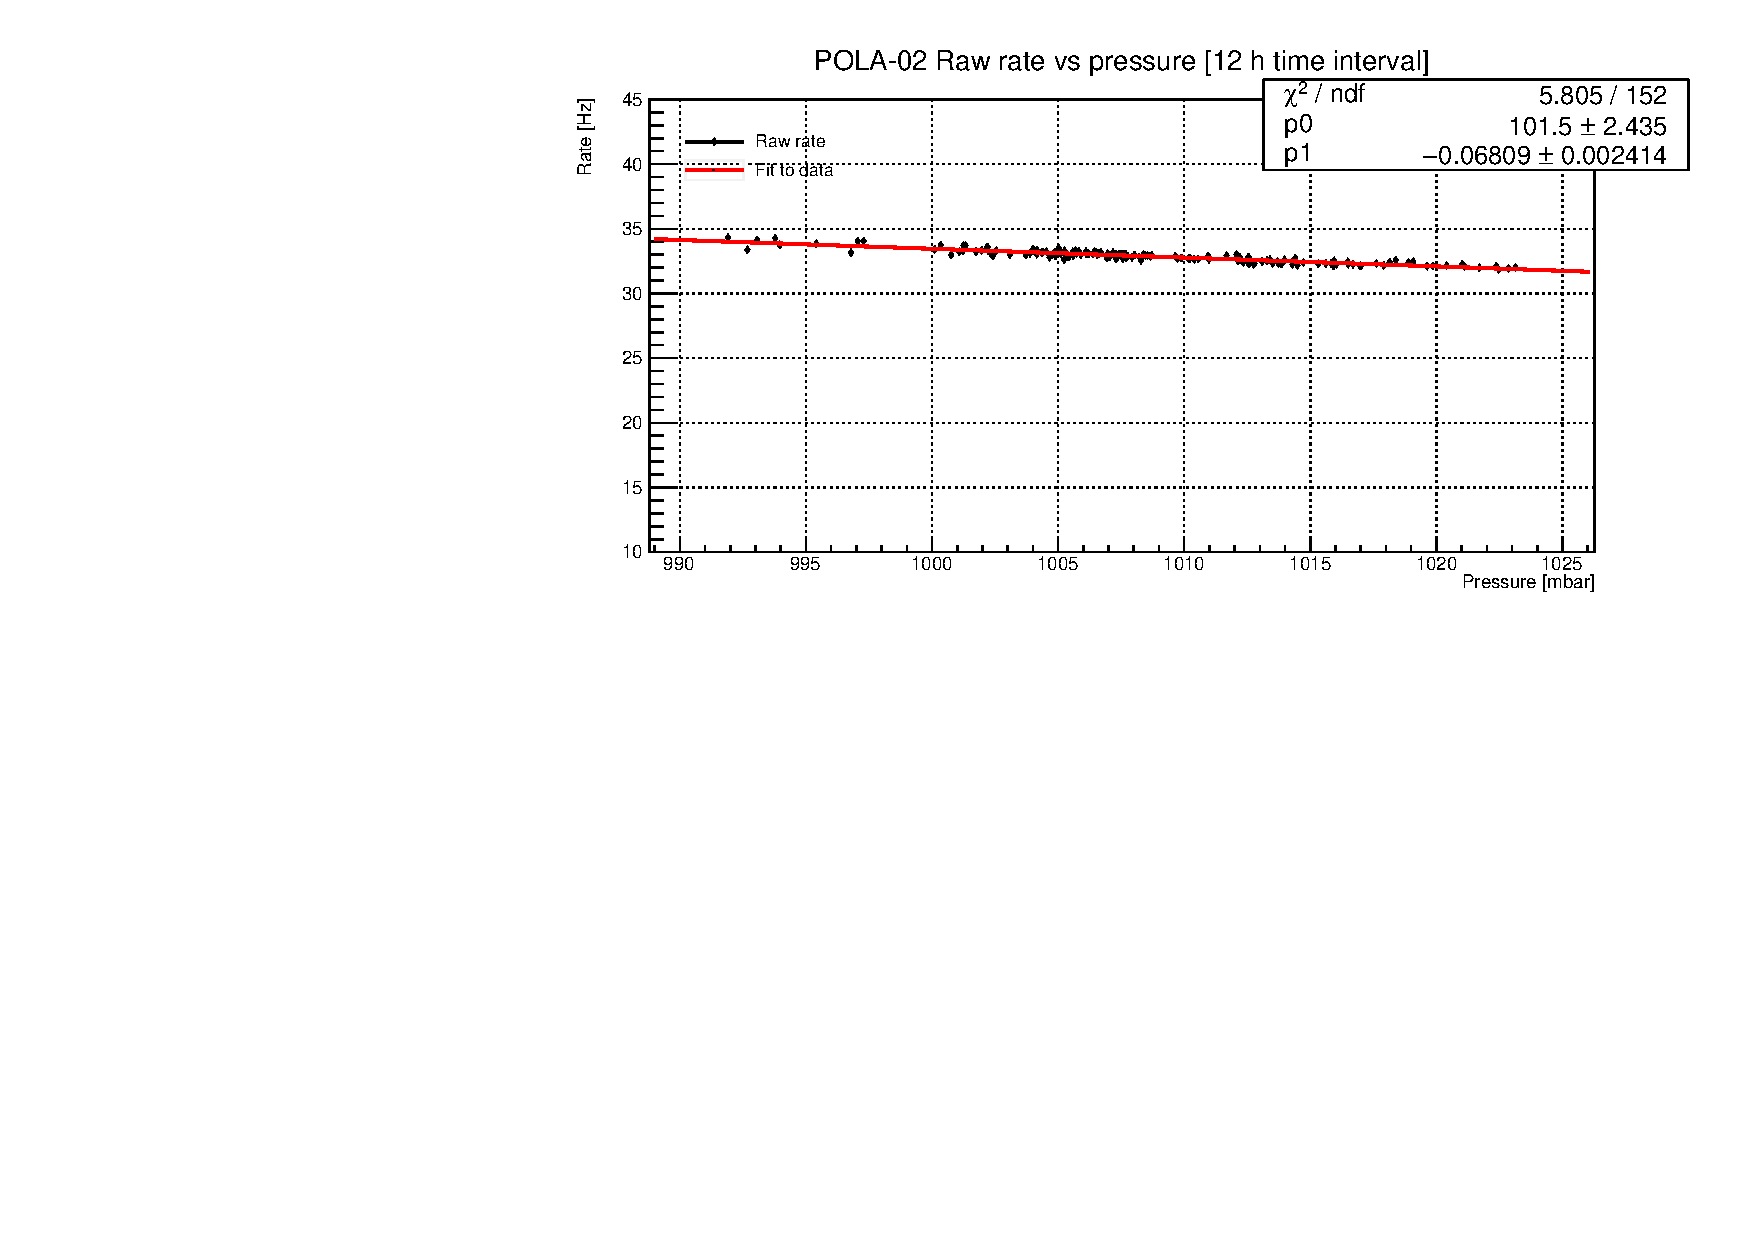
\includegraphics[width=0.5\textwidth]{figures/fixed_POLA02_rate_pressure_fit.pdf}}
    \hspace{0.5cm}
    \subfloat[POLA-03]{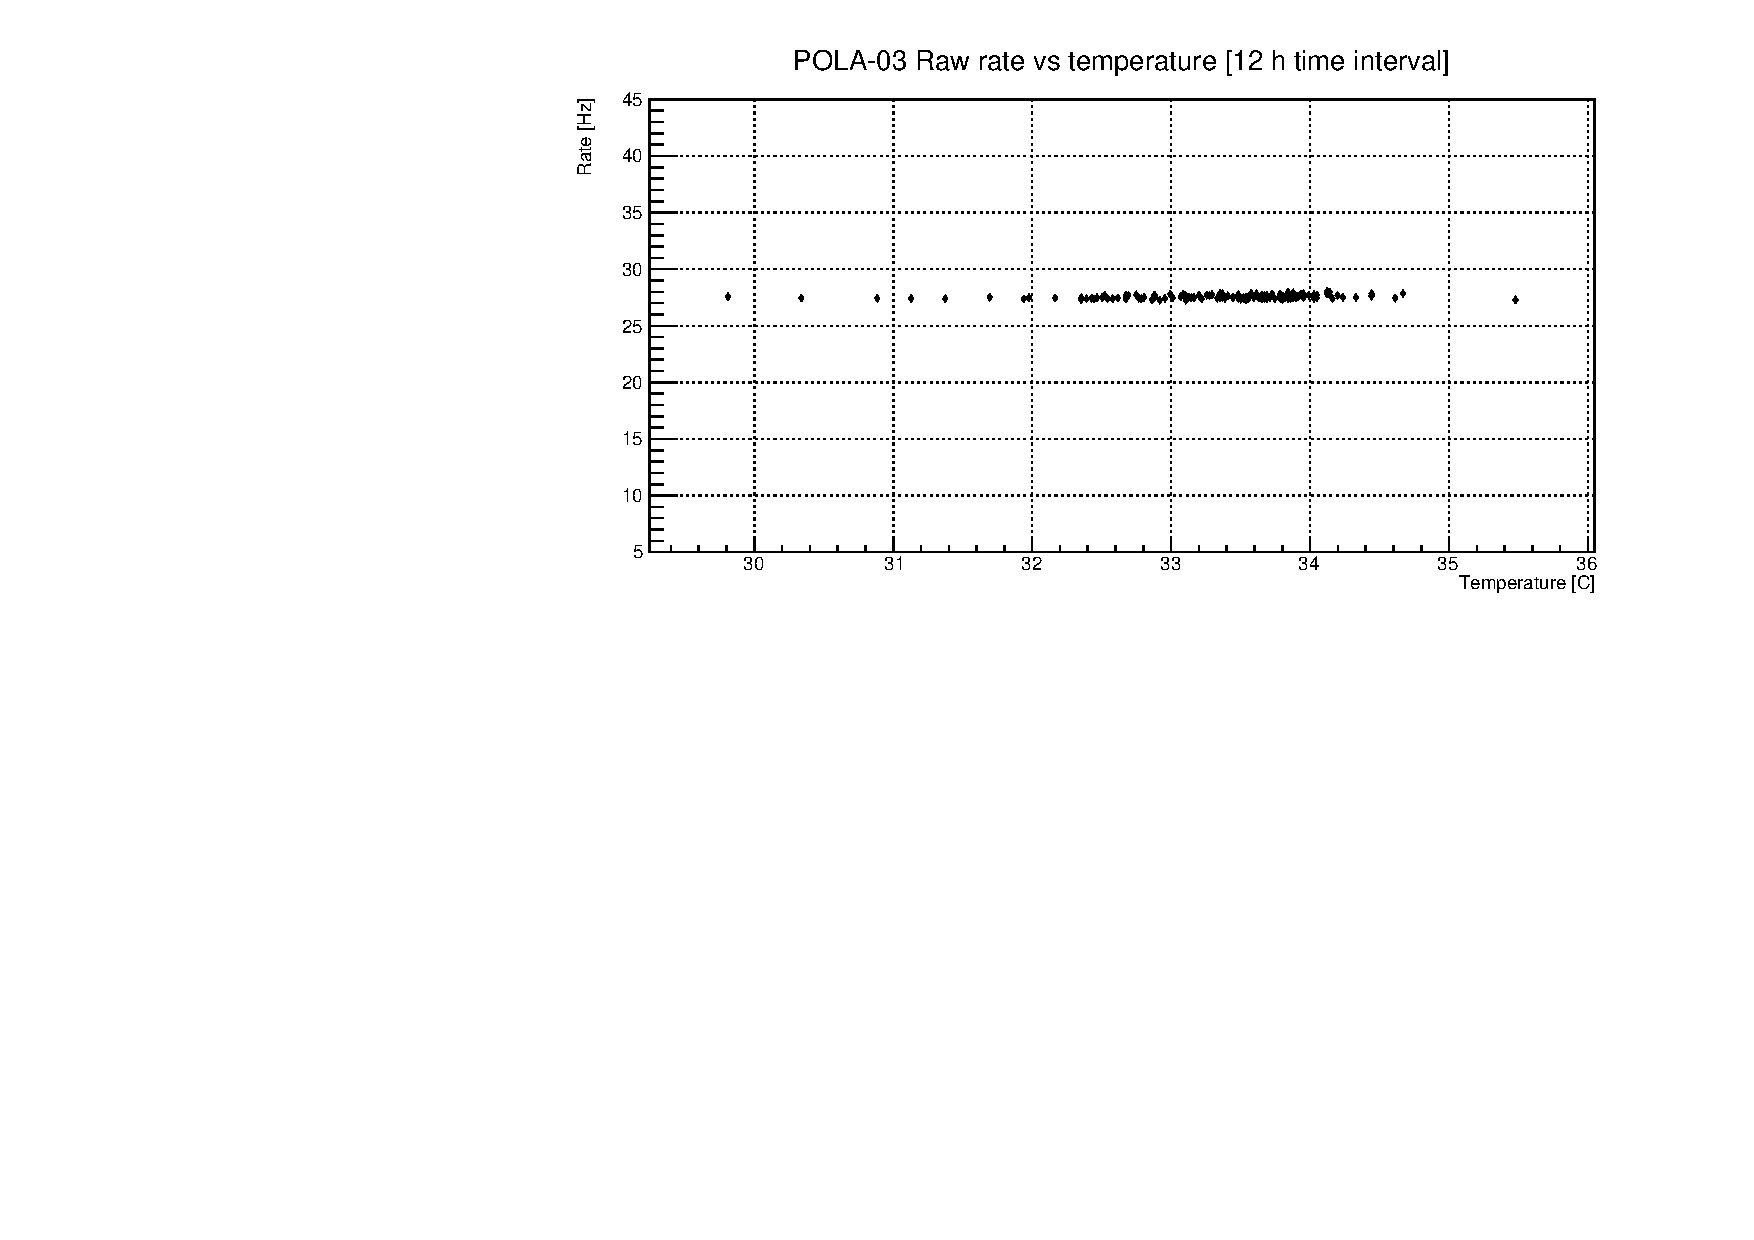
\includegraphics[width=0.5\textwidth]{figures/fixed_POLA03_rate_temp_fit.pdf}}
    \subfloat[POLA-03]{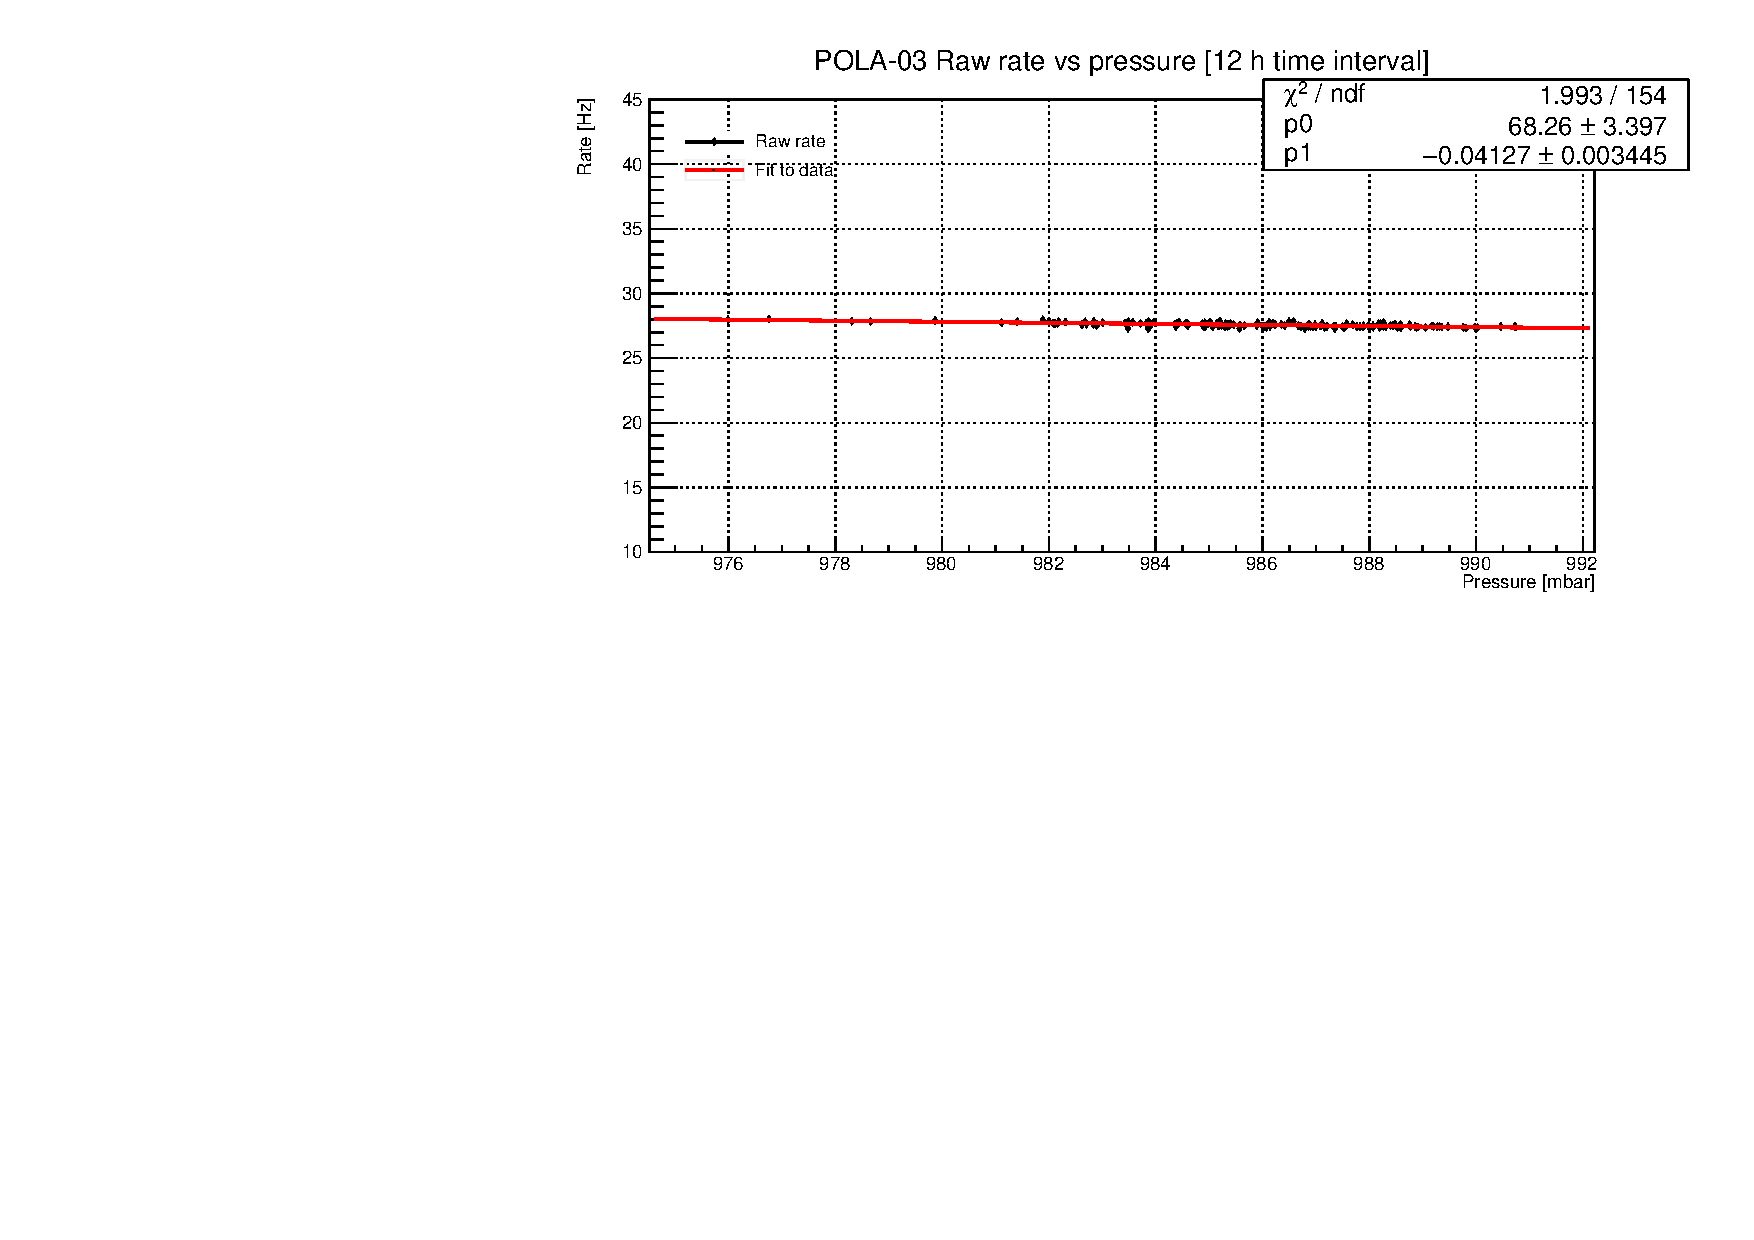
\includegraphics[width=0.5\textwidth]{figures/fixed_POLA03_rate_pressure_fit.pdf}}
    \caption{Plots on the left show the uncorrected raw rate as a function of temperature and on the right the uncorrected raw rate as a function of pressure. The red line shows the linear fit of the data.}
    \label{fig:raw_temp_press_all}
\end{figure}

\newpage

\bibliography{ref}

\end{document}